\documentclass[12pt]{article}
\usepackage{sbc-template}
\usepackage{graphicx,url}
\IfFileExists{brazil.ldf}{\usepackage[brazil]{babel}}{\usepackage[english]{babel}\addto\captionsenglish{\renewcommand{\figurename}{Figura}\renewcommand{\tablename}{Tabela}\renewcommand{\refname}{Refer\^encias}}\hyphenpenalty=10000\exhyphenpenalty=10000}
\usepackage[utf8]{inputenc}
\usepackage[T1]{fontenc}
\usepackage{amsmath,amssymb}
\usepackage{booktabs}
\usepackage{array}
\newcolumntype{L}[1]{>{\raggedright\arraybackslash}p{#1}}
\sloppy


\newcommand{\solN}{56}
\newcommand{\solGapMedio}{1.49}
\newcommand{\solGapMediana}{1.30}
\newcommand{\solGapMax}{4.95}
\newcommand{\solIgual}{17}
\newcommand{\solTempoTotal}{160}
\newcommand{\solTempoMedio}{2.9}
\newcommand{\solVerificadas}{56}
\newcommand{\solVeicSolver}{480}
\newcommand{\solVeicBks}{483}
\newcommand{\solPior}{C204}
\newcommand{\tabSolomon}{
\begin{tabular}{lrrrrr}
\toprule
Família & Inst. & Dif. média (\%) & Dif. máx. (\%) & Veículos (nós / BKS) & Tempo (s) \\
\midrule
C1 & 9 & 0.00 & 0.00 & 90 / 90 & 2.2 \\
C2 & 8 & 1.24 & 4.95 & 26 / 24 & 3.4 \\
R1 & 12 & 1.87 & 4.95 & 160 / 159 & 3.1 \\
R2 & 11 & 1.88 & 4.23 & 56 / 60 & 3.0 \\
RC1 & 8 & 1.72 & 2.26 & 102 / 100 & 2.6 \\
RC2 & 8 & 2.11 & 4.78 & 46 / 50 & 3.0 \\
\bottomrule
\end{tabular}
}
\newcommand{\xGapMedio}{2.10}
\newcommand{\xGapMax}{3.92}
\newcommand{\xVerificadas}{9}
\newcommand{\xN}{9}
\newcommand{\tabCvrp}{
\begin{tabular}{lrrrrrr}
\toprule
Instância & Cl. & BKS & Solver & Dif. (\%) & Veíc. & Tempo (s) \\
\midrule
X-n101-k25 & 100 & 27591 & 27968 & 1.37 & 26 / 26 & 1.24 \\
X-n106-k14 & 105 & 26362 & 26717 & 1.35 & 14 / 14 & 1.19 \\
X-n120-k6 & 119 & 13332 & 13571 & 1.79 & 6 / 6 & 1.92 \\
X-n129-k18 & 128 & 28940 & 29736 & 2.75 & 18 / 18 & 1.32 \\
X-n153-k22 & 152 & 21220 & 21521 & 1.42 & 24 / 23 & 2.11 \\
X-n190-k8 & 189 & 16980 & 17293 & 1.84 & 8 / 8 & 2.82 \\
X-n209-k16 & 208 & 30656 & 31264 & 1.98 & 16 / 16 & 1.76 \\
X-n251-k28 & 250 & 38684 & 39628 & 2.44 & 28 / 28 & 2.22 \\
X-n303-k21 & 302 & 21736 & 22589 & 3.92 & 21 / 21 & 2.99 \\
\bottomrule
\end{tabular}
}
\newcommand{\tabAblacao}{
\begin{tabular}{lrrrrr}
\toprule
Instância & BKS & Econ. & Inserção & + Busca local & + Ruína e recr. \\
\midrule
C101 & 827.3 & 12.2 & 0.0 & 0.0 & 0.0 \\
C201 & 589.1 & 27.2 & 0.0 & 0.0 & 0.0 \\
R101 & 1637.7 & 21.9 & 19.1 & 3.7 & 0.0 \\
R201 & 1143.2 & 23.7 & 47.1 & 17.5 & 0.5 \\
RC101 & 1619.8 & 30.4 & 21.5 & 7.5 & 1.3 \\
RC201 & 1261.8 & 40.5 & 75.2 & 35.3 & 1.9 \\
X-n101-k25 & 27591.0 & 6.8 & 14.3 & 5.6 & 1.4 \\
X-n153-k22 & 21220.0 & 6.2 & 24.6 & 5.7 & 1.4 \\
\bottomrule
\end{tabular}
}
\newcommand{\ablConstrMin}{0.0}
\newcommand{\ablConstrMax}{40.5}
\newcommand{\ablLocalMin}{0.0}
\newcommand{\ablLocalMax}{35.3}
\newcommand{\ablFinalMin}{0.0}
\newcommand{\ablFinalMax}{1.9}
\newcommand{\ablNuncaPiorou}{sim}
\newcommand{\expConstr}{2.2}
\newcommand{\expIter}{0.7}
\newcommand{\expViario}{1.8}
\newcommand{\expCompleto}{1.3}
\newcommand{\tabEscala}{
\begin{tabular}{rrrrrrr}
\toprule
$n$ & Arcos (completo) & Arcos (viário) & Grafo completo & Viário + Dijkstra & Constr. + busca local & 1000 iter. \\
\midrule
25 & 650 & 160 & 0.003 & 0.002 & 0.003 & 0.091 \\
50 & 2550 & 310 & 0.001 & 0.003 & 0.007 & 0.132 \\
100 & 10100 & 606 & 0.004 & 0.012 & 0.03 & 0.162 \\
150 & 22650 & 922 & 0.008 & 0.027 & 0.078 & 0.193 \\
200 & 40200 & 1218 & 0.015 & 0.055 & 0.13 & 0.278 \\
300 & 90300 & 1836 & 0.032 & 0.126 & 0.523 & 0.621 \\
400 & 160400 & 2374 & 0.055 & 0.237 & 1.476 & 0.753 \\
\bottomrule
\end{tabular}
}
\newcommand{\escalaTodasVerificadas}{sim}
\newcommand{\viarioAcrescimoMedio}{27.9}
\newcommand{\viarioAcrescimoMin}{21.6}
\newcommand{\viarioAcrescimoMax}{35.9}
\newcommand{\viarioN}{6}
\newcommand{\viarioVerificadas}{6}
\newcommand{\viarioArcosCompleto}{6480}
\newcommand{\viarioArcosViario}{494}
\newcommand{\tabViario}{
\begin{tabular}{rrrrr}
\toprule
Semente & Dist. completo & Dist. viário & Acréscimo (\%) & Veíc. (compl. / viário) \\
\midrule
0 & 1931.53 & 2399.56 & 24.2 & 16 / 16 \\
1 & 1630.65 & 1982.17 & 21.6 & 14 / 14 \\
2 & 1718.03 & 2334.39 & 35.9 & 14 / 14 \\
3 & 1712.42 & 2307.78 & 34.8 & 15 / 15 \\
4 & 1893.83 & 2370.34 & 25.2 & 15 / 15 \\
5 & 1828.96 & 2300.79 & 25.8 & 16 / 15 \\
\bottomrule
\end{tabular}
}
\newcommand{\tabPrioridade}{
\begin{tabular}{lrrrrr}
\toprule
Cenário & $\lambda$ & Dist. média & Início (alta) & Início (baixa) & $\sum w\,s$ \\
\midrule
com janelas & 0.0 & 1436.25 & 292.53 & 270.06 & 26796.0 \\
com janelas & 0.5 & 1511.84 & 279.92 & 264.92 & 25941.0 \\
com janelas & 1.0 & 1564.48 & 279.79 & 264.24 & 25894.0 \\
com janelas & 2.0 & 1579.47 & 279.75 & 263.6 & 25864.0 \\
com janelas & 5.0 & 1645.55 & 279.6 & 263.42 & 25855.0 \\
sem janelas & 0.0 & 1243.7 & 78.8 & 82.64 & 7957.0 \\
sem janelas & 0.5 & 1364.53 & 53.9 & 75.08 & 6102.0 \\
sem janelas & 1.0 & 1418.78 & 54.19 & 72.32 & 5977.0 \\
sem janelas & 2.0 & 1453.03 & 52.35 & 72.73 & 5964.0 \\
sem janelas & 5.0 & 1464.86 & 51.58 & 72.71 & 5953.0 \\
\bottomrule
\end{tabular}
}
\newcommand{\prioInstancias}{5}
\newcommand{\prioPesoMax}{5.0}
\newcommand{\prioJanAltaZero}{292.53}
\newcommand{\prioJanAltaMax}{279.6}
\newcommand{\prioJanBaixaZero}{270.06}
\newcommand{\prioJanBaixaMax}{263.42}
\newcommand{\prioJanDistZero}{1436.25}
\newcommand{\prioJanDistMax}{1645.55}
\newcommand{\prioJanPondZero}{26796.0}
\newcommand{\prioJanPondMax}{25855.0}
\newcommand{\prioJanDistPct}{14.6}
\newcommand{\prioJanPondPct}{3.5}
\newcommand{\prioSemAltaZero}{78.8}
\newcommand{\prioSemAltaMax}{51.58}
\newcommand{\prioSemBaixaZero}{82.64}
\newcommand{\prioSemBaixaMax}{72.71}
\newcommand{\prioSemDistZero}{1243.7}
\newcommand{\prioSemDistMax}{1464.86}
\newcommand{\prioSemPondZero}{7957.0}
\newcommand{\prioSemPondMax}{5953.0}
\newcommand{\prioSemDistPct}{17.8}
\newcommand{\prioSemPondPct}{25.2}
\newcommand{\exN}{50}
\newcommand{\exOtimas}{50}
\newcommand{\exGapMedio}{0.00}
\newcommand{\exGapMax}{0.00}
\newcommand{\exTempoExato}{0.7}
\newcommand{\exTempoHeur}{0.1}
\newcommand{\tabGH}{
\begin{tabular}{lrrrrrr}
\toprule
Instância & Veíc. & BKS veíc. & Distância & BKS dist. & Dif. (\%) & Tempo (s) \\
\midrule
c1\_2\_1 & 20 & 20 & 2704.57 & 2704.57 & 0.00 & 0.3 \\
c2\_2\_1 & 6 & 6 & 1931.44 & 1931.44 & 0.00 & 0.6 \\
r1\_2\_1 & 26 & 20 & 4835.71 & 4784.11 & --- & 1.0 \\
r2\_2\_1 & 14 & 4 & 3567.43 & 4483.16 & --- & 1.1 \\
rc1\_2\_1 & 22 & 18 & 3800.37 & 3602.80 & --- & 0.5 \\
rc2\_2\_1 & 11 & 6 & 2877.43 & 3099.53 & --- & 0.9 \\
\bottomrule
\end{tabular}
}
\newcommand{\ghN}{30}
\newcommand{\ghVerificadas}{30}
\newcommand{\ghCompletas}{12}
\newcommand{\ghMelhoriaMin}{0.4}
\newcommand{\ghMelhoriaMax}{36.9}
\newcommand{\ghBuscaMelhoriaMin}{0.1}
\newcommand{\ghBuscaMelhoriaMax}{39.2}
\newcommand{\ghTempoMaxBusca}{188}
\newcommand{\ghTempoMaxCompleto}{7}
\newcommand{\tabEntregas}{
\begin{tabular}{rrrrrrrr}
\toprule
Entregas & $\lambda$ & Dist. (km) & Veíc. & Atraso alta (min) & Atraso média (min) & Atraso baixa (min) & Tempo (s) \\
\midrule
100 & 0.0 & 557 & 6 & 188 & 208 & 191 & 0.5 \\
100 & 0.01 & 587 & 6 & 57 & 91 & 116 & 0.9 \\
100 & 0.05 & 720 & 7 & 3 & 3 & 48 & 1.4 \\
200 & 0.0 & 845 & 12 & 146 & 231 & 237 & 1.2 \\
200 & 0.01 & 944 & 12 & 42 & 76 & 114 & 2.8 \\
200 & 0.05 & 1183 & 11 & 10 & 7 & 33 & 4.5 \\
500 & 0.0 & 1649 & 29 & 228 & 246 & 229 & 8.6 \\
500 & 0.01 & 1872 & 31 & 23 & 40 & 74 & 40.3 \\
500 & 0.05 & 2340 & 26 & 7 & 12 & 25 & 25.6 \\
\bottomrule
\end{tabular}
}
\newcommand{\entAltaBase}{146}
\newcommand{\entAltaPrio}{42}
\newcommand{\entDistPct}{11.7}
\newcommand{\entAltaBaseQ}{228}
\newcommand{\entAltaPrioQ}{23}
\newcommand{\entDistPctQ}{13.5}
\newcommand{\entViarioPct}{34.6}
\newcommand{\entVerificadas}{13}
\newcommand{\entN}{13}
\newcommand{\entMil}{61}
\newcommand{\entMilTempo}{50}


\title{Roteamento e Carga de Veículos em Centros Logísticos:\\ uma ferramenta baseada em grafos}

\author{João Gabriel Maia da Costa\inst{1}, Thomas Ramos Oliveira\inst{1},\\ Pedro Eduardo Pimenta\inst{1}}

\address{Engenharia de Software\\ Pontifícia Universidade Católica de Minas Gerais (PUC Minas)\\ Teoria dos Grafos -- Trabalho Prático, Tema 10}

\begin{document}
\maketitle

\begin{abstract}
This paper presents a graph-based tool that plans logistics routes under vehicle capacity, time-window, distance and priority constraints. Vehicle routes are circuits in a weighted directed graph that can be complete or a sparse road network, in which Dijkstra's algorithm provides the costs. The solver combines the savings and Solomon insertion heuristics with local search and a ruin-and-recreate metaheuristic, and every solution is checked by an independent verifier. On \solN{} Solomon instances the total distance is on average \solGapMedioEn\% above the best known solutions, and on \xN{} larger capacitated instances it is \xGapMedioEn\% above. The tool has a web interface and no graph library.
\end{abstract}

\begin{resumo}
Este trabalho apresenta uma ferramenta, baseada em grafos, que planeja rotas logísticas com restrições de capacidade dos veículos, janelas de tempo, distância e prioridade. As rotas são circuitos em um grafo dirigido ponderado, que pode ser completo ou uma rede viária esparsa, na qual o algoritmo de Dijkstra fornece os custos. O solver combina as heurísticas de economias e de inserção de Solomon com busca local e uma metaheurística de ruína e recriação, e toda solução é conferida por um verificador independente. Em \solN{} instâncias de Solomon, a distância total fica em média \solGapMedio\% acima das melhores soluções conhecidas, e em \xN{} instâncias maiores com capacidade fica \xGapMedio\% acima. Ela também roda dados do Kaggle: instâncias de Gehring e Homberger e 1000 entregas de e-commerce. A ferramenta tem interface web e não usa biblioteca de grafos.
\end{resumo}

\section{Introdução}

Um centro logístico decide todos os dias quais veículos saem do depósito, que clientes cada um atende e em que ordem. A decisão muda o custo de transporte, o número de veículos usados, o cumprimento dos horários combinados e o atendimento dos pedidos urgentes. Esse é o problema de roteamento de veículos, estudado desde a década de 1950 \cite{dantzig1959,tothvigo2014}. Ele generaliza o caixeiro viajante e é NP-difícil \cite{lenstra1981}, de modo que instâncias reais pedem heurísticas.

Este trabalho trata do Tema 10 da disciplina: \emph{roteamento e carga de veículos em centros logísticos, com restrições de tempo, distância, prioridade e capacidade de carga}. O objetivo é construir uma ferramenta que modele o problema como grafo, aplique algoritmos compatíveis com ele, mostre os resultados em uma interface gráfica e permita avaliar correção, complexidade e limitações. As contribuições são:
\begin{itemize}
  \item um modelo em grafo dirigido com dois modos, completo e rede viária, com caminhos mínimos por Dijkstra;
  \item um solver que mantém toda solução viável e respeita as quatro restrições do tema;
  \item uma validação em camadas: testes, verificador independente, solver exato e melhores soluções conhecidas;
  \item uma avaliação experimental reproduzível, com sementes e iterações fixas.
\end{itemize}
Estrutura, algoritmos e verificação são implementados pelo grupo em Python, só com a biblioteca padrão. Nenhuma biblioteca de grafos é usada, nem mesmo para comparação de desempenho. A Seção~2 define o problema, a Seção~3 apresenta a modelagem, a Seção~4 os algoritmos e a complexidade, a Seção~5 a implementação, a Seção~6 a validação, a Seção~7 os resultados e as Seções~8 e 9 as limitações e conclusões.

\section{Definição do problema e dados}

Há um depósito (vértice $0$) e clientes $C=\{1,\dots,n\}$. O cliente $i$ tem demanda $q_i$, janela de tempo $[e_i,l_i]$, tempo de serviço $\sigma_i$ e prioridade $p_i\in\{1,2,3\}$ (alta, média, baixa). Os veículos são idênticos, com capacidade $Q$, no máximo $K$ disponíveis e, opcionalmente, distância máxima $D_{\max}$ por rota. Uma rota $r=(0,i_1,\dots,i_m,0)$ é viável quando:
\begin{itemize}
  \item \textbf{capacidade:} $\sum_k q_{i_k}\le Q$;
  \item \textbf{tempo:} com $s_{i_k}=\max\bigl(e_{i_k},\,s_{i_{k-1}}+\sigma_{i_{k-1}}+t_{i_{k-1}i_k}\bigr)$ e $s_{i_0}=e_0$, vale $s_{i_k}\le l_{i_k}$, e o retorno ocorre até $l_0$; chegar cedo obriga a esperar;
  \item \textbf{distância:} $d(r)\le D_{\max}$, quando houver limite.
\end{itemize}
A \textbf{prioridade} entra no objetivo, para que clientes urgentes sejam atendidos mais cedo sem tornar o problema inviável. Busca-se um conjunto de no máximo $K$ rotas viáveis que cubra todos os clientes e minimize
\begin{equation}
\sum_{r\in R}\bigl(F+d(r)\bigr)+\lambda\sum_{i\in C}w_{p_i}\,s_i,
\label{eq:obj}
\end{equation}
com custo fixo $F\ge0$, peso $\lambda\ge0$ e $w_1=3$, $w_2=2$, $w_3=1$. Com $F=\lambda=0$ o objetivo é a distância total, a mesma das melhores soluções publicadas.

\textbf{Dados.} Foram usadas quatro fontes. As duas primeiras são benchmarks da literatura com melhor solução conhecida (BKS), o que permite medir a qualidade do resultado: as 56 instâncias de Solomon \cite{solomon1987}, com 100 clientes, capacidade e janelas de tempo, e 9 instâncias do conjunto X \cite{uchoa2017}, de 101 a 303 clientes, sem janelas. Os arquivos vêm do repositório público PyVRP/Instances (licença MIT), que os reproduz do CVRPLIB, no formato VRPLIB. As distâncias de Solomon são truncadas na primeira casa decimal e as do conjunto X arredondadas ao inteiro; o leitor aplica a mesma convenção, e o verificador reproduz exatamente o custo das 65 BKS. As outras duas vêm do Kaggle: o conjunto \emph{VRPTW Benchmark Datasets} \cite{kagglevrptw}, licença CC BY 4.0, com as 300 instâncias de Gehring e Homberger \cite{gehring1999} de 200 a 1000 clientes e janelas de tempo, e o \emph{E-commerce Logistics Route Planning Dataset} \cite{kaggleecom}, licença CC0, com 1000 entregas urbanas, com latitude, longitude, peso, janela de tempo e prioridade. Instâncias sintéticas, com semente fixa, completam os testes de escala, rede viária, prioridade e comparação com o solver exato.

\section{Modelagem em grafos}

O sistema usa um grafo dirigido ponderado $G=(V,A,d,t)$ com $V=\{0,\dots,n\}$ e, para cada arco $(u,v)$, uma distância $d_{uv}$ e um tempo $t_{uv}$. Uma rota é um circuito de $G$ pelo depósito, e uma solução é uma partição de $C$ em no máximo $K$ circuitos. A estrutura é dirigida porque distâncias e tempos podem ser assimétricos (ruas de mão única). Ela é central: todos os algoritmos leem os custos do grafo, o verificador confere que cada trecho de rota existe nele, e o modo viário depende de caminhos mínimos sobre ele.

\begin{figure}[!ht]
\centering
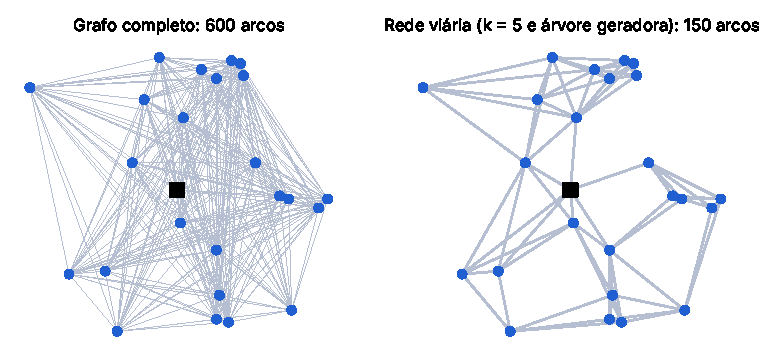
\includegraphics[width=0.7\linewidth]{figuras/fig_modos_grafo.pdf}
\caption{Os dois modos do grafo para a mesma instância sintética de 24 clientes (quadrado preto: depósito).}
\label{fig:modos}
\end{figure}

A Figura~\ref{fig:modos} mostra os modos. No \textbf{modo completo} há um arco entre todo par de pontos, com peso igual à distância euclidiana arredondada pela regra da base; ele é o modelo padrão da literatura e permite comparar com as BKS. No \textbf{modo viário} cada ponto liga-se aos $k=5$ vizinhos mais próximos e as arestas de uma árvore geradora mínima (Kruskal com union-find) garantem conexidade. Cada aresta recebe um desvio aleatório de 0 a 30\% sobre a distância em linha reta, e uma fração opcional das arestas pode ter mão única. Os custos entre clientes são os caminhos mínimos por Dijkstra, e o trajeto físico de cada rota é reconstruído e desenhado no mapa. Antes de resolver, uma busca em largura no grafo e no seu transposto detecta clientes sem caminho de ida e volta ao depósito, e a instância é recusada com mensagem clara.

\begin{figure}[!ht]
\centering
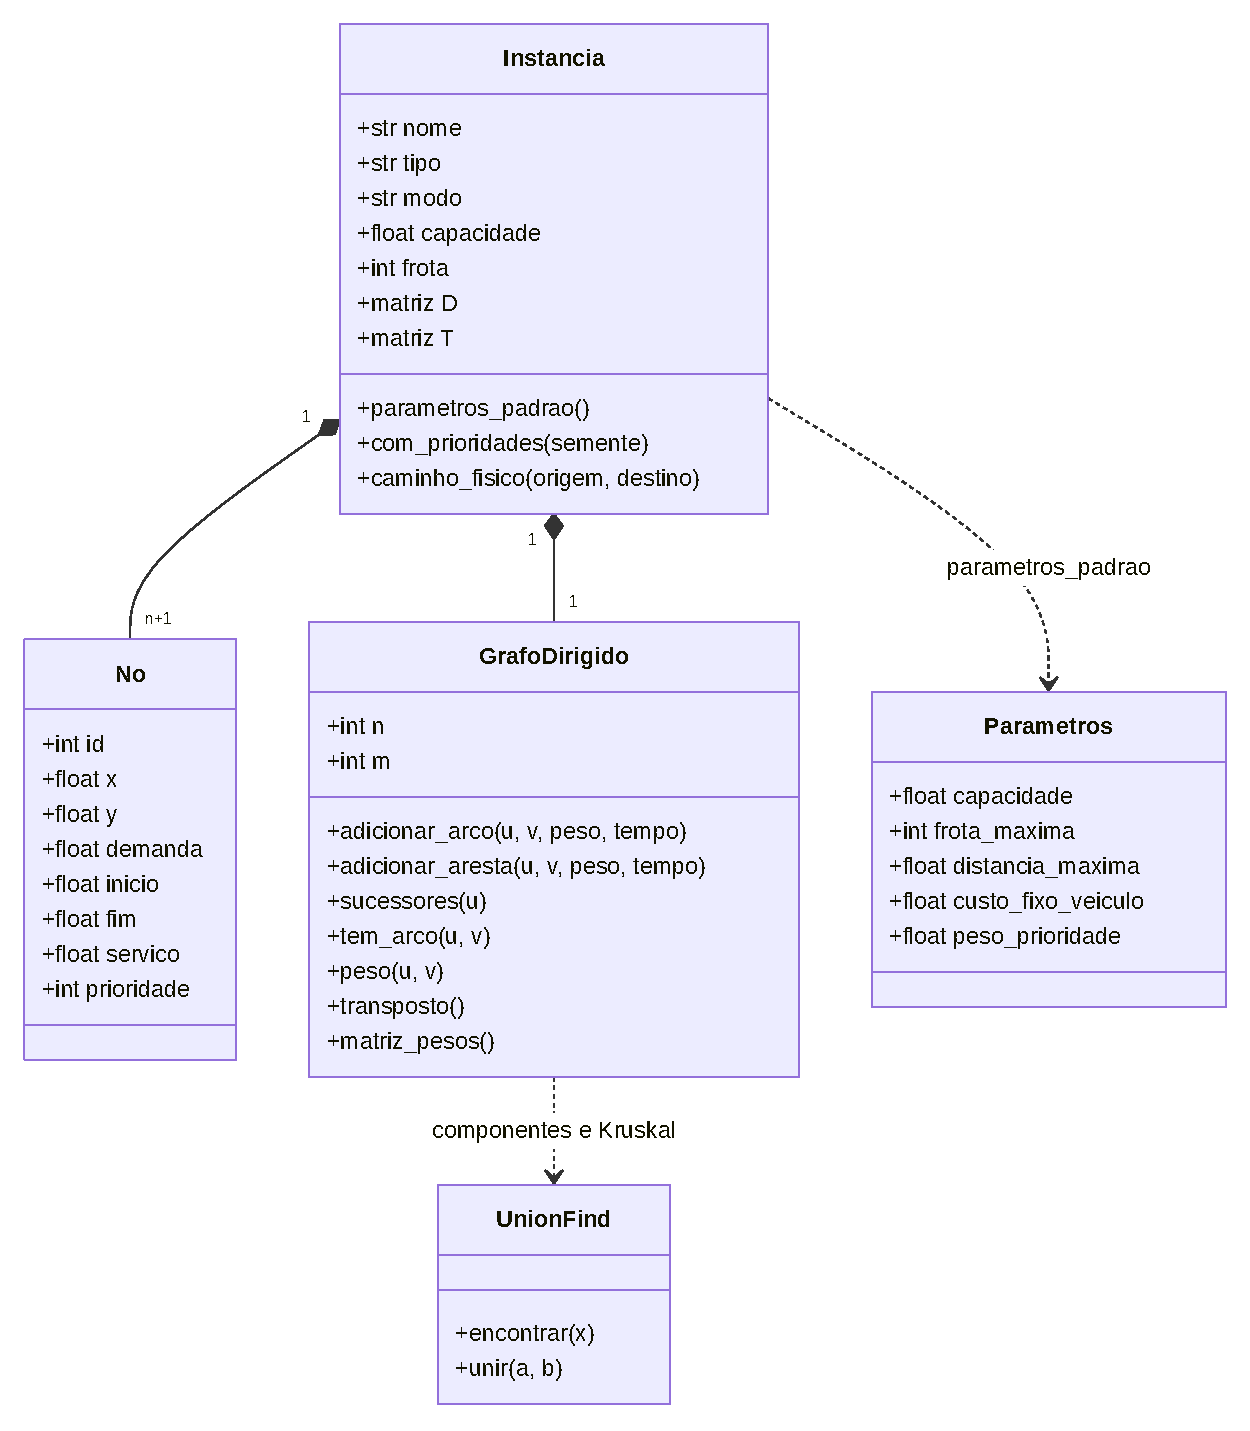
\includegraphics[width=0.45\linewidth]{../docs/diagramas/classes_modelo.pdf}\\[4pt]
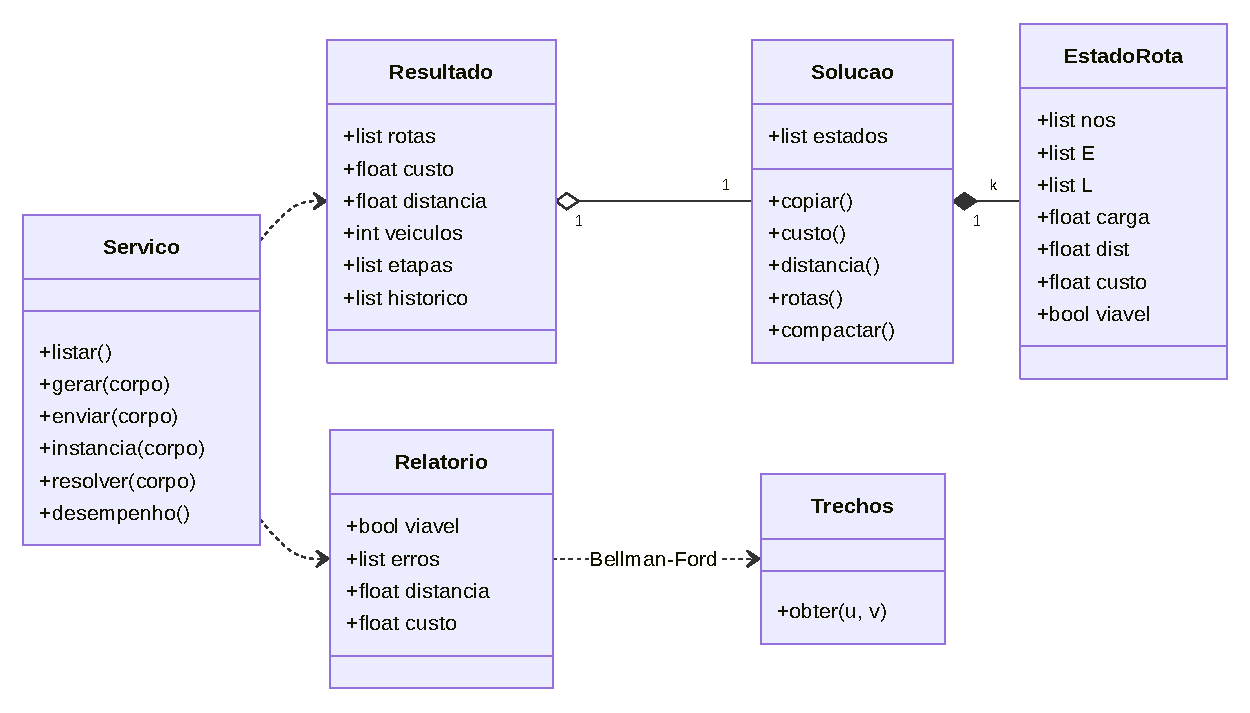
\includegraphics[width=0.8\linewidth]{../docs/diagramas/classes_execucao.pdf}
\caption{Diagramas de classes: modelo e grafo (acima) e solução, resultado e verificação (abaixo). Os algoritmos são funções de módulo.}
\label{fig:classes}
\end{figure}

\begin{figure}[!ht]
\centering
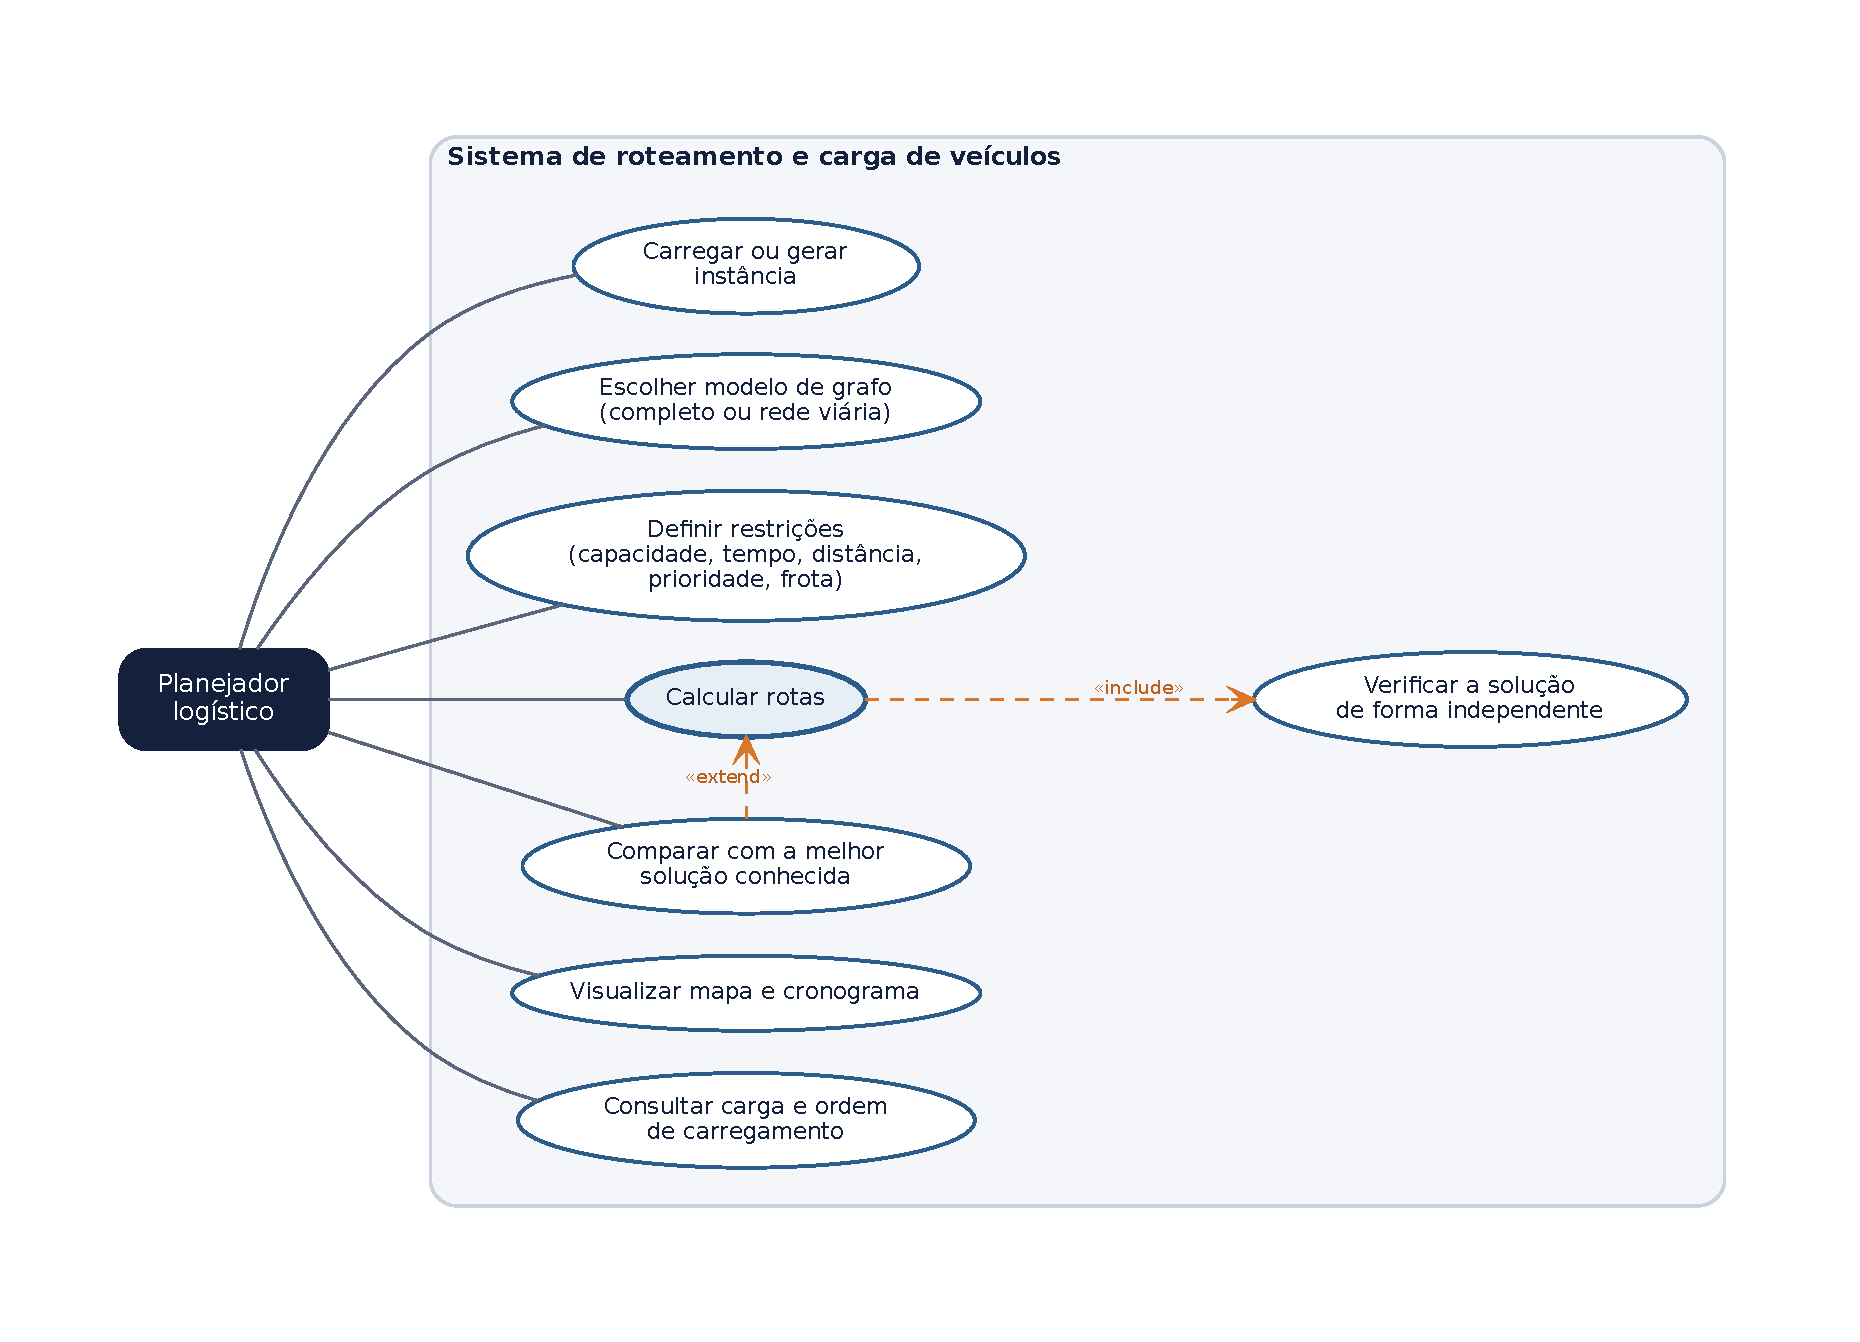
\includegraphics[width=0.62\linewidth]{../docs/diagramas/casos_de_uso.pdf}
\caption{Diagrama de casos de uso.}
\label{fig:casos}
\end{figure}

\begin{figure}[!ht]
\centering
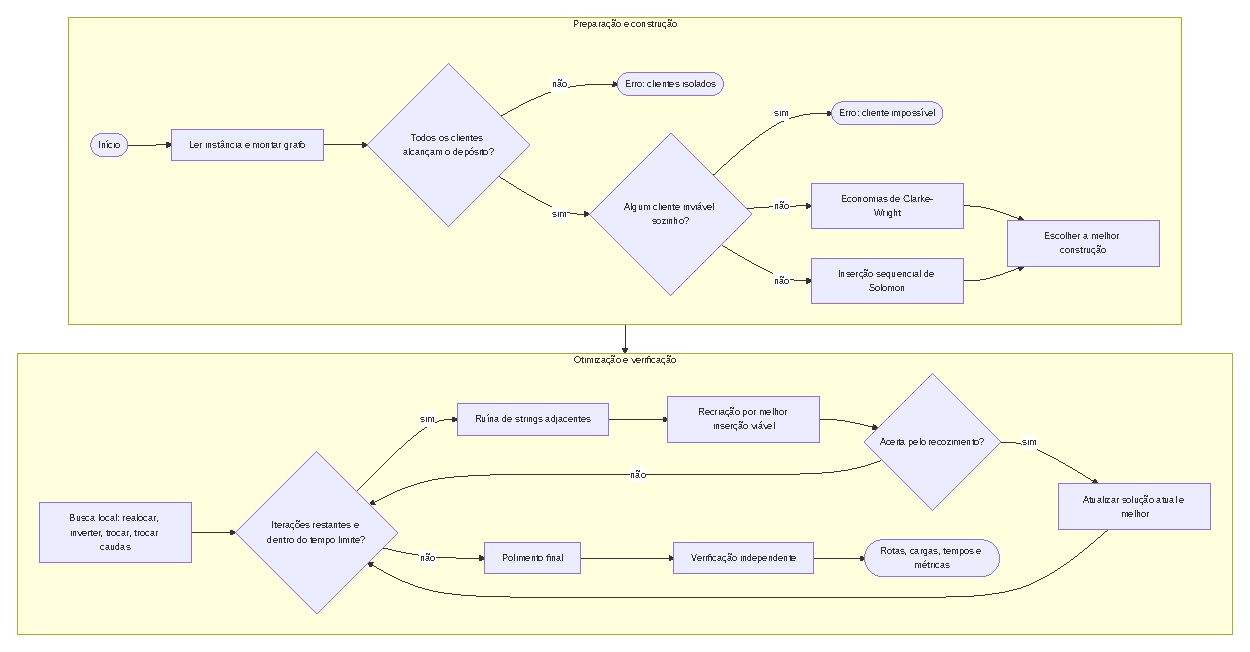
\includegraphics[width=0.8\linewidth]{../docs/diagramas/atividades.pdf}
\caption{Diagrama de atividades do solver, da leitura da instância à verificação independente.}
\label{fig:ativ}
\end{figure}

As Figuras~\ref{fig:classes}, \ref{fig:casos} e~\ref{fig:ativ} mostram as classes, os casos de uso e o fluxo de atividades do solver, e as Figuras~\ref{fig:comp} e~\ref{fig:seq}, a arquitetura em componentes e a sequência de uma solicitação. Os diagramas completos da Etapa 1 estão em \texttt{docs/}. A Figura~\ref{fig:comp} mostra também que a interface web só se comunica com o solver por uma API JSON, o que permite trocar a interface sem alterar a lógica de otimização, e que cada frente de trabalho tem testes próprios.

\begin{figure}[!ht]
\centering
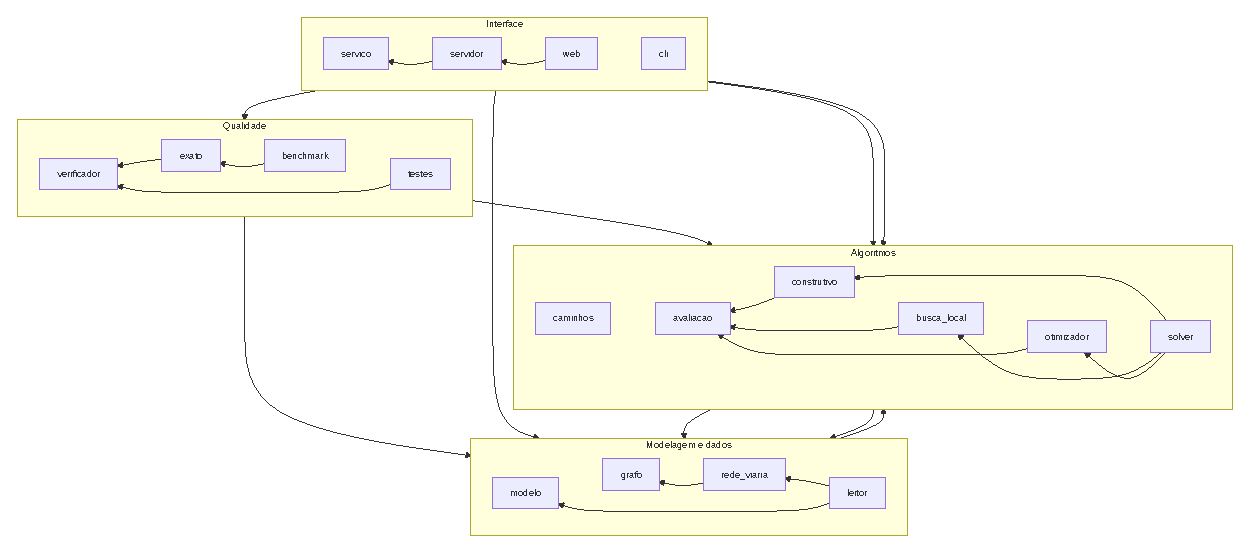
\includegraphics[width=0.82\linewidth]{../docs/diagramas/componentes.pdf}
\caption{Diagrama de componentes, agrupado pelas quatro frentes de trabalho.}
\label{fig:comp}
\end{figure}

\begin{figure}[!ht]
\centering
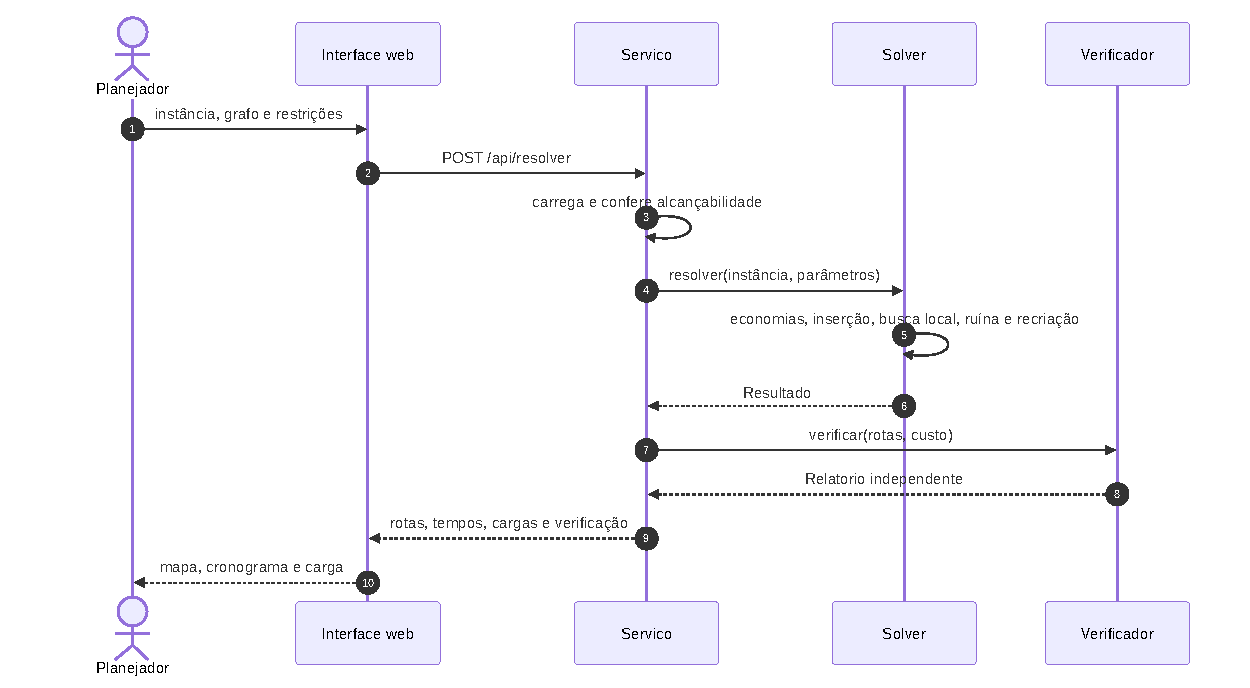
\includegraphics[width=0.72\linewidth]{../docs/diagramas/sequencia.pdf}
\caption{Diagrama de sequência do cálculo de rotas pela interface.}
\label{fig:seq}
\end{figure}

\section{Algoritmos e complexidade}

Seja $n$ o número de clientes, $m$ o de arcos, $R$ o de rotas e $L$ o tamanho da maior rota. Nas expressões seguintes, o custo de cada algoritmo é dado em função desses parâmetros. No modo completo, $m=n(n+1)$; no modo viário, $m=O(kn)$, com $k=5$ vizinhos por vértice. Os limites são de pior caso e omitem constantes, que pesam em Python.

\textbf{Dijkstra.} Com heap binário, um caminho mínimo de uma origem custa $O((n+m)\log n)$ \cite{dijkstra1959,clrs2009}. Os pesos são não negativos, condição de correção do algoritmo, e o construtor do grafo rejeita pesos negativos. No modo viário, $m=O(kn)$, e as $n+1$ origens custam $O(kn^2\log n)$. No modo completo o arco direto já é o caminho mínimo e a matriz é lida diretamente, sem Dijkstra.

\textbf{Conexidade.} Kruskal com union-find \cite{kruskal1956} custa $O(m\log m)$; aqui as candidatas são todos os pares, logo $O(n^2\log n)$. A alcançabilidade usa duas buscas em largura, $O(n+m)$. Os componentes fracamente conexos, usados no diagnóstico, também custam $O(n+m)$. Na prática, isso permite recusar de imediato uma instância cuja rede deixe algum cliente isolado, em vez de descobrir o problema no meio da otimização.

\textbf{Avaliação de rotas em tempo constante.} Para cada rota guardamos o início mais cedo $E_k$ de cada posição e o início mais tarde $L_k$ que ainda mantém viável o restante da rota \cite{savelsbergh1985}. Inserir $u$ entre $p$ e $x$ é viável se, e somente se, a carga cabe, o início em $u$ respeita $l_u$ e o novo início em $x$ não passa de $L_x$. A condição é suficiente porque o atraso se propaga monotonicamente pela rota e $L_x$ resume a folga de todo o sufixo. Cada posição custa $O(1)$ e recalcular uma rota custa $O(L)$. Com $\lambda>0$ o efeito da inserção nos instantes de início é propagado até o ponto em que a espera o absorve.

\textbf{Soluções iniciais.} As economias de Clarke-Wright \cite{clarke1964} ordenam os $O(n^2)$ pares por ganho $d_{0i}+d_{j0}-d_{ij}$ e fundem rotas quando a fusão é viável: $O(n^2\log n)$ para ordenar e $O(L)$ por teste. A inserção sequencial de Solomon \cite{solomon1987} abre uma rota com o cliente mais difícil e insere repetidamente o cliente de melhor critério em sua melhor posição viável: $O(n^2L)$. O solver executa as duas e parte da melhor.

\textbf{Busca local.} As vizinhanças são realocação, troca, troca de caudas entre rotas e inversão de trecho. Antes da avaliação completa, que custa $O(L)$, cada candidato passa por filtros $O(1)$: carga e distância por somas de prefixo e janelas pelas folgas $E$ e $L$; só segue quem não é claramente inviável ou pior. No pior caso a troca e as caudas continuam $O(n^2L)$ por passada e a inversão $O(nL^2)$, mas na prática quase todo candidato é descartado em $O(1)$. Os filtros não mudam os movimentos aceitos: as rotas são idênticas às da avaliação completa, o que um teste confere, e a busca local ficou de 2 a 8 vezes mais rápida (em 400 entregas, de 16,5\,s para 2,1\,s). Cada movimento só é aplicado se a solução resultante é viável e estritamente melhor, o que garante terminação; a busca para no primeiro ótimo local e é executada antes e depois da ruína e recriação.

\textbf{Ruína e recriação.} Em cada iteração removem-se trechos contíguos de rotas próximas a um cliente sorteado, em média cerca de dez clientes, no estilo de \cite{christiaens2020}; os removidos são reinseridos pela melhor posição viável, com pequena probabilidade de ignorar posições para diversificar, e abre-se uma rota nova apenas se não houver inserção viável. A solução candidata só é considerada se todos os removidos voltaram, de modo que toda solução intermediária é viável. A aceitação usa recozimento simulado \cite{kirkpatrick1983}, com temperatura decrescente de forma geométrica. Uma iteração custa $O(n)$ no total, com constante em torno do número de removidos, e a ordenação das vizinhanças é feita uma vez em $O(n^2\log n)$. A execução é determinística dada a semente e o número de iterações.

\textbf{Verificação independente e solver exato.} O verificador não reutiliza as matrizes do solver: recalcula as distâncias das coordenadas e, no modo viário, usa Bellman-Ford, $O(nm)$ por origem. O solver exato enumera as permutações de todo subconjunto, $O(n\cdot n!)$, e combina as rotas por programação dinâmica sobre máscaras, $O(3^n)$; por isso o código o limita a 9 clientes, e os experimentos usam instâncias de 8. Como os dois caminhos de cálculo não compartilham código, um erro de modelagem do solver não se repete no verificador, e os testes comparam os dois em todas as instâncias de referência.

\textbf{Memória.} O custo de espaço é dominado pelas matrizes de distância e de tempo, $O(n^2)$, que o grafo completo e as tabelas de caminhos mínimos exigem; no modo viário a lista de adjacência tem só $O(kn)$ arcos, mas a matriz e os predecessores de Dijkstra continuam $O(n^2)$. A lista de economias também tem $O(n^2)$ pares. Cada rota guarda $O(L)$ valores de $E$ e $L$, a solução inteira ocupa $O(n)$, e a busca local e a ruína e recriação só alteram essa solução. O solver exato guarda $O(2^n)$ subconjuntos. Medimos o pico de memória do processo em instâncias sintéticas: 19, 28, 70 e 249\,MB para 100, 200, 400 e 800 clientes, crescimento coerente com $O(n^2)$ somado ao custo fixo do interpretador.

\section{Implementação e interface}

O código e o histórico de desenvolvimento estão em \url{https://github.com/Joaogabrielmaia/Tp-Logistica}. O sistema tem cerca de 3\,100 linhas (2\,300 em Python e 780 em HTML, CSS e JavaScript), sem dependências externas e com comentários curtos apenas nos pontos não óbvios dos algoritmos. A Figura~\ref{fig:comp} mostra a separação em quatro grupos: modelagem e dados, algoritmos, interface e qualidade. A interface é uma página web servida localmente pela biblioteca padrão, e se comunica com o solver por uma API JSON que valida todas as entradas (tamanho de arquivo, limites de iterações, parâmetros inválidos, caminhos fora da pasta de dados). Pela linha de comando também é possível resolver instâncias e rodar os experimentos.

As Figuras~\ref{fig:telas1} e~\ref{fig:telas2} mostram as telas, obtidas com a ferramenta em execução. O mapa desenha as rotas sobre o grafo, com prioridade alta e média destacadas; o cronograma mostra, para cada veículo, janelas de tempo, esperas e atendimentos; a tela de carga mostra a ocupação de cada veículo e a ordem de carregamento (o último cliente entregue é o primeiro a entrar); a convergência mostra a evolução do custo e a contribuição de cada etapa. Toda solução exibida traz o resultado da verificação independente.

\begin{figure}[!ht]
\centering
\begin{minipage}{0.495\linewidth}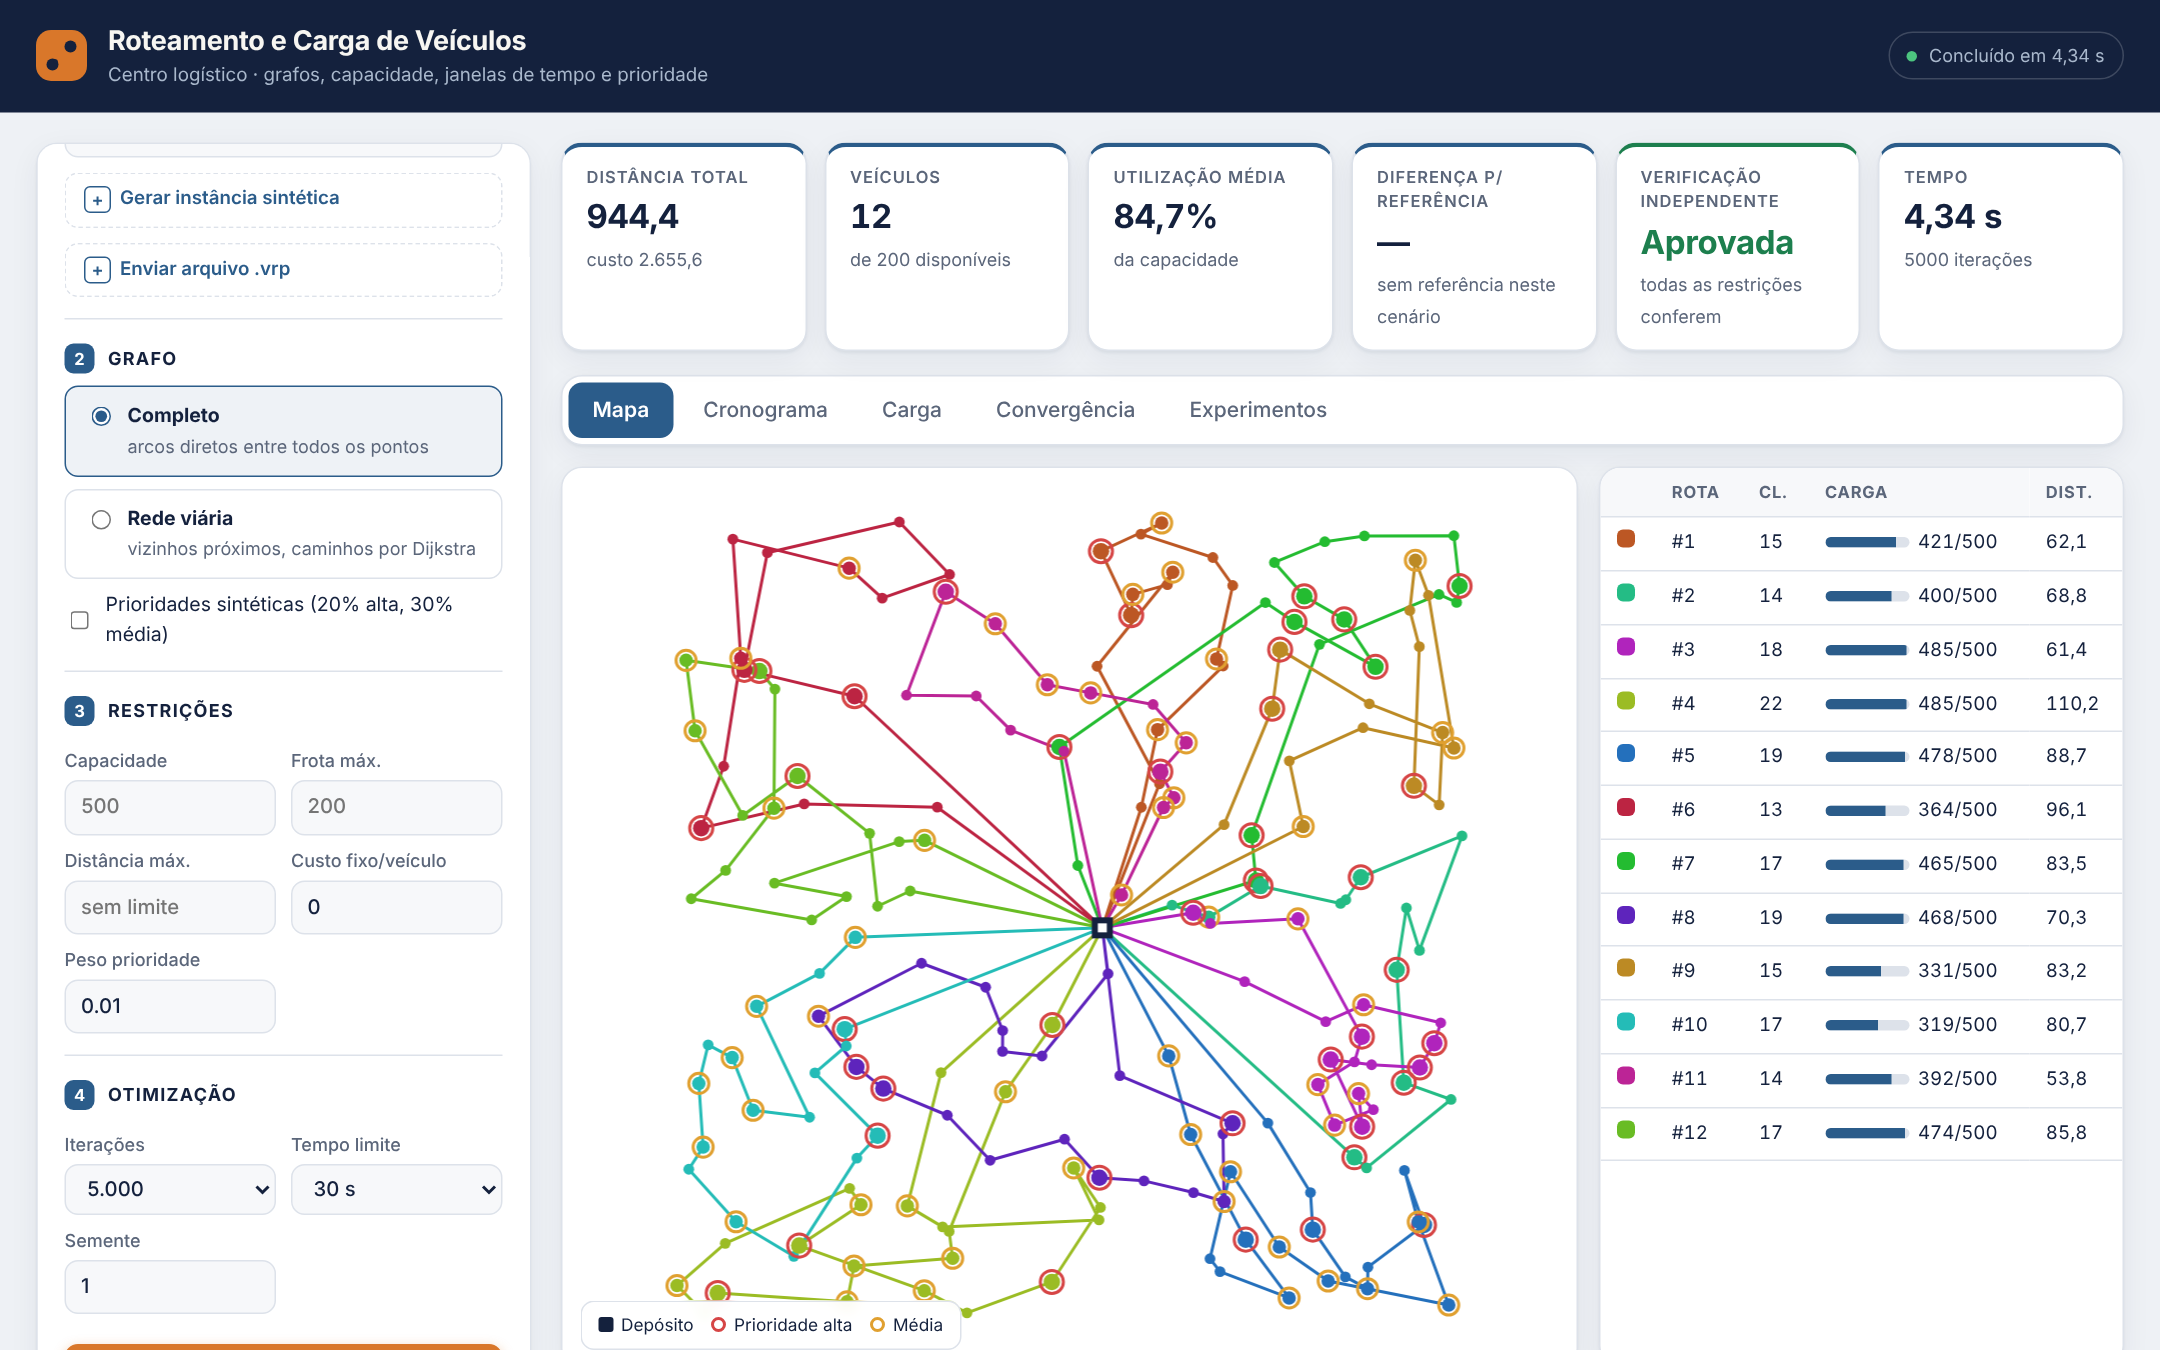
\includegraphics[width=\linewidth]{figuras/tela_mapa.png}\end{minipage}
\begin{minipage}{0.495\linewidth}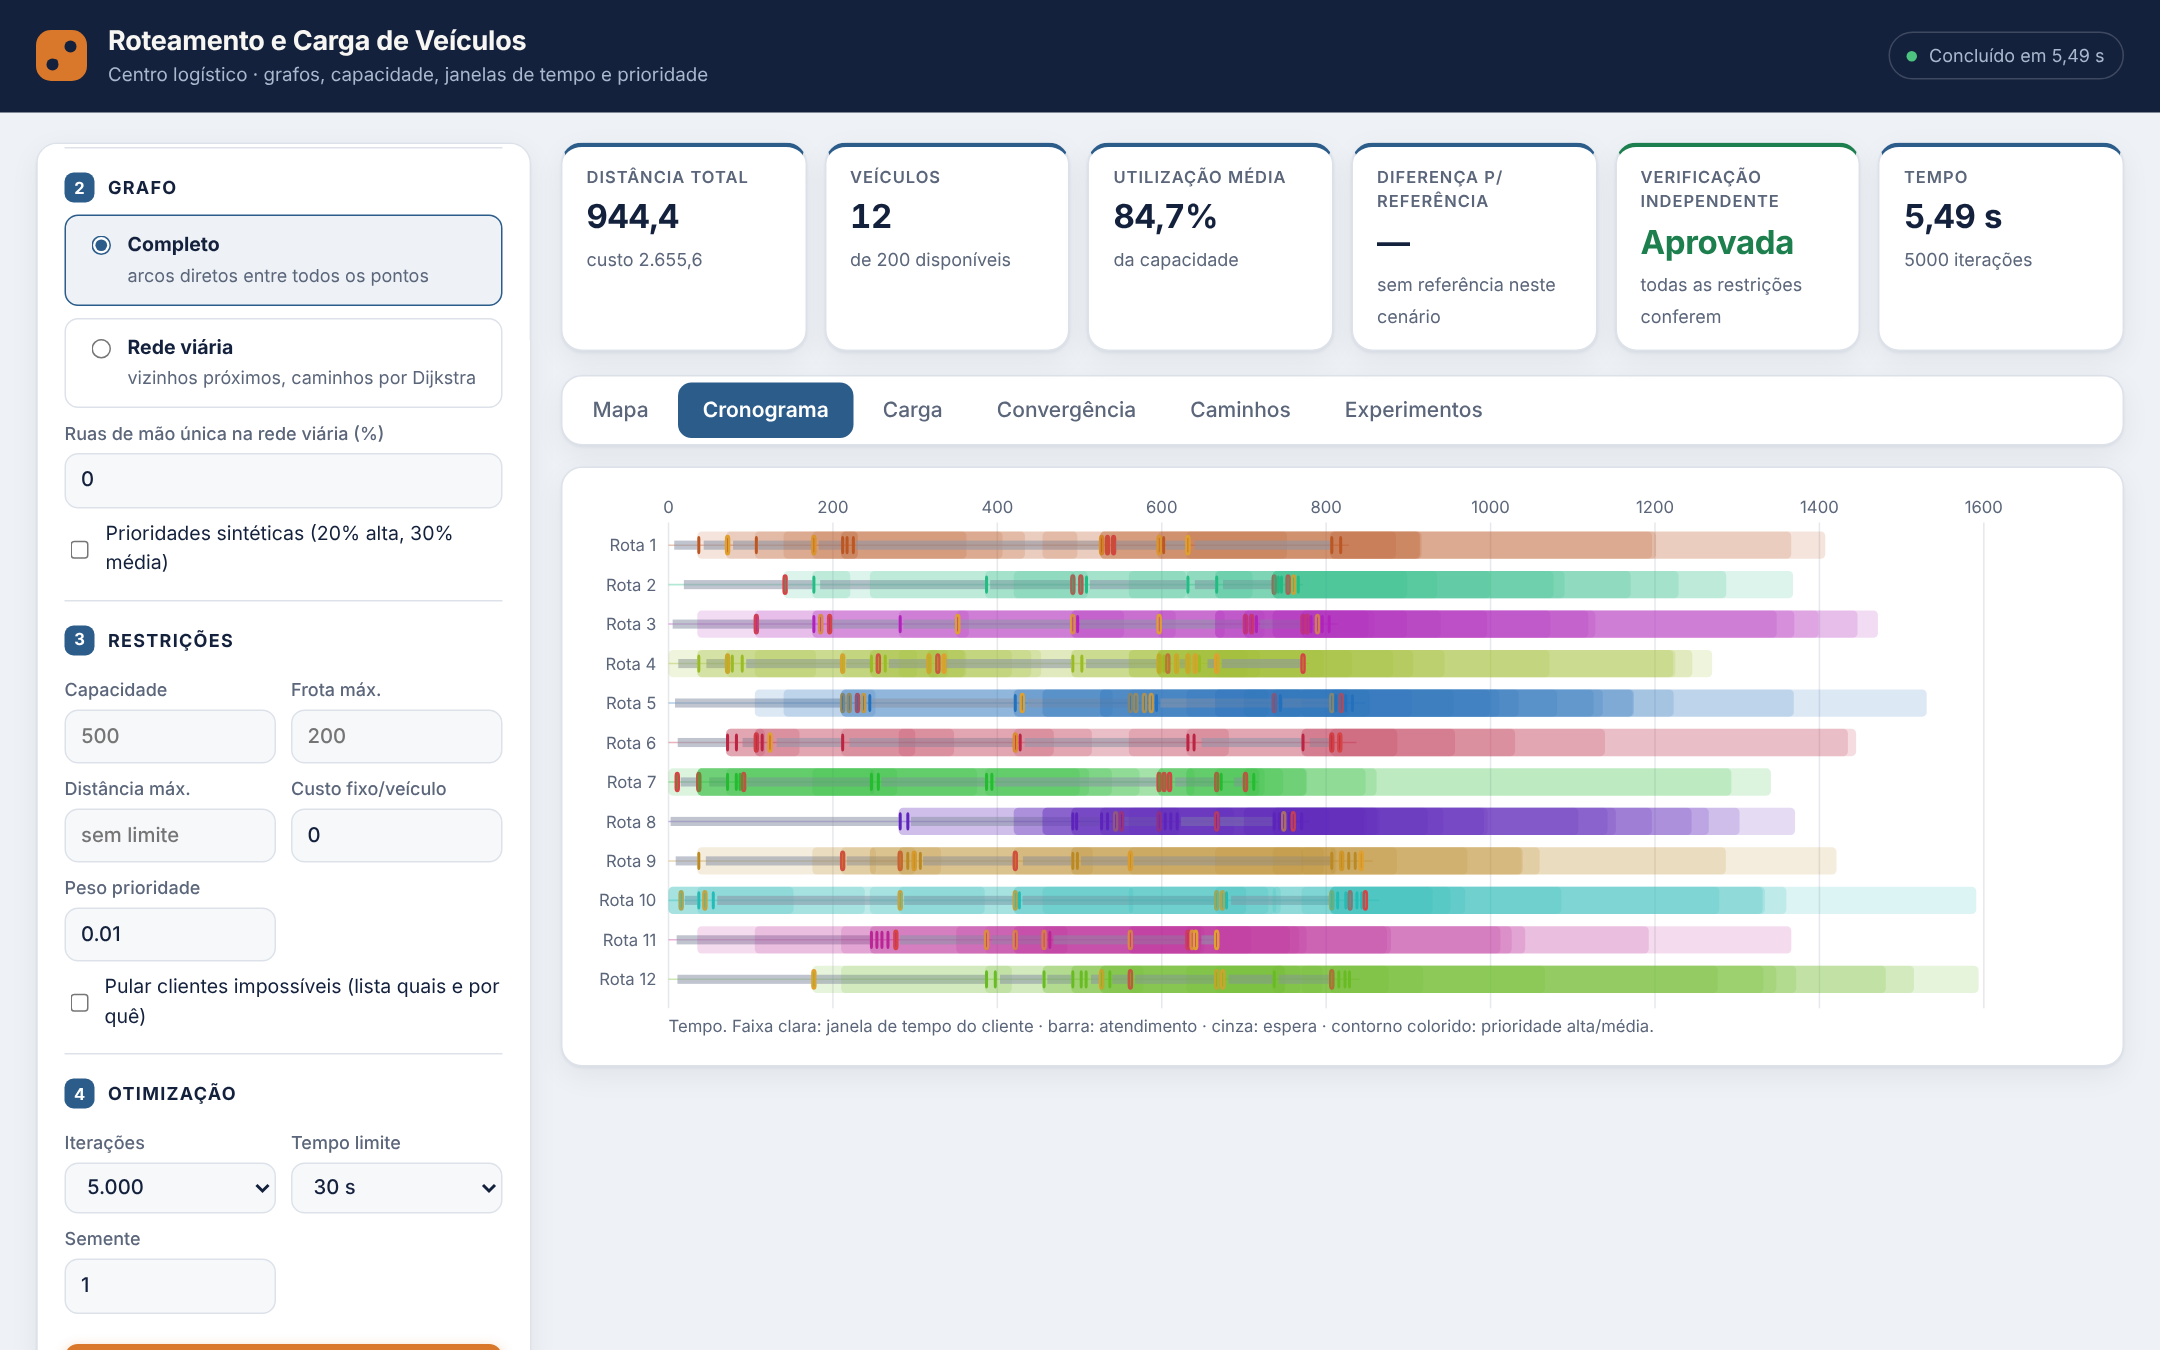
\includegraphics[width=\linewidth]{figuras/tela_cronograma.png}\end{minipage}
\caption{Mapa (à esquerda) e cronograma por veículo (à direita) para 200 entregas do Kaggle, com peso de prioridade $\lambda=0{,}01$.}
\label{fig:telas1}
\end{figure}

\begin{figure}[!ht]
\centering
\begin{minipage}{0.325\linewidth}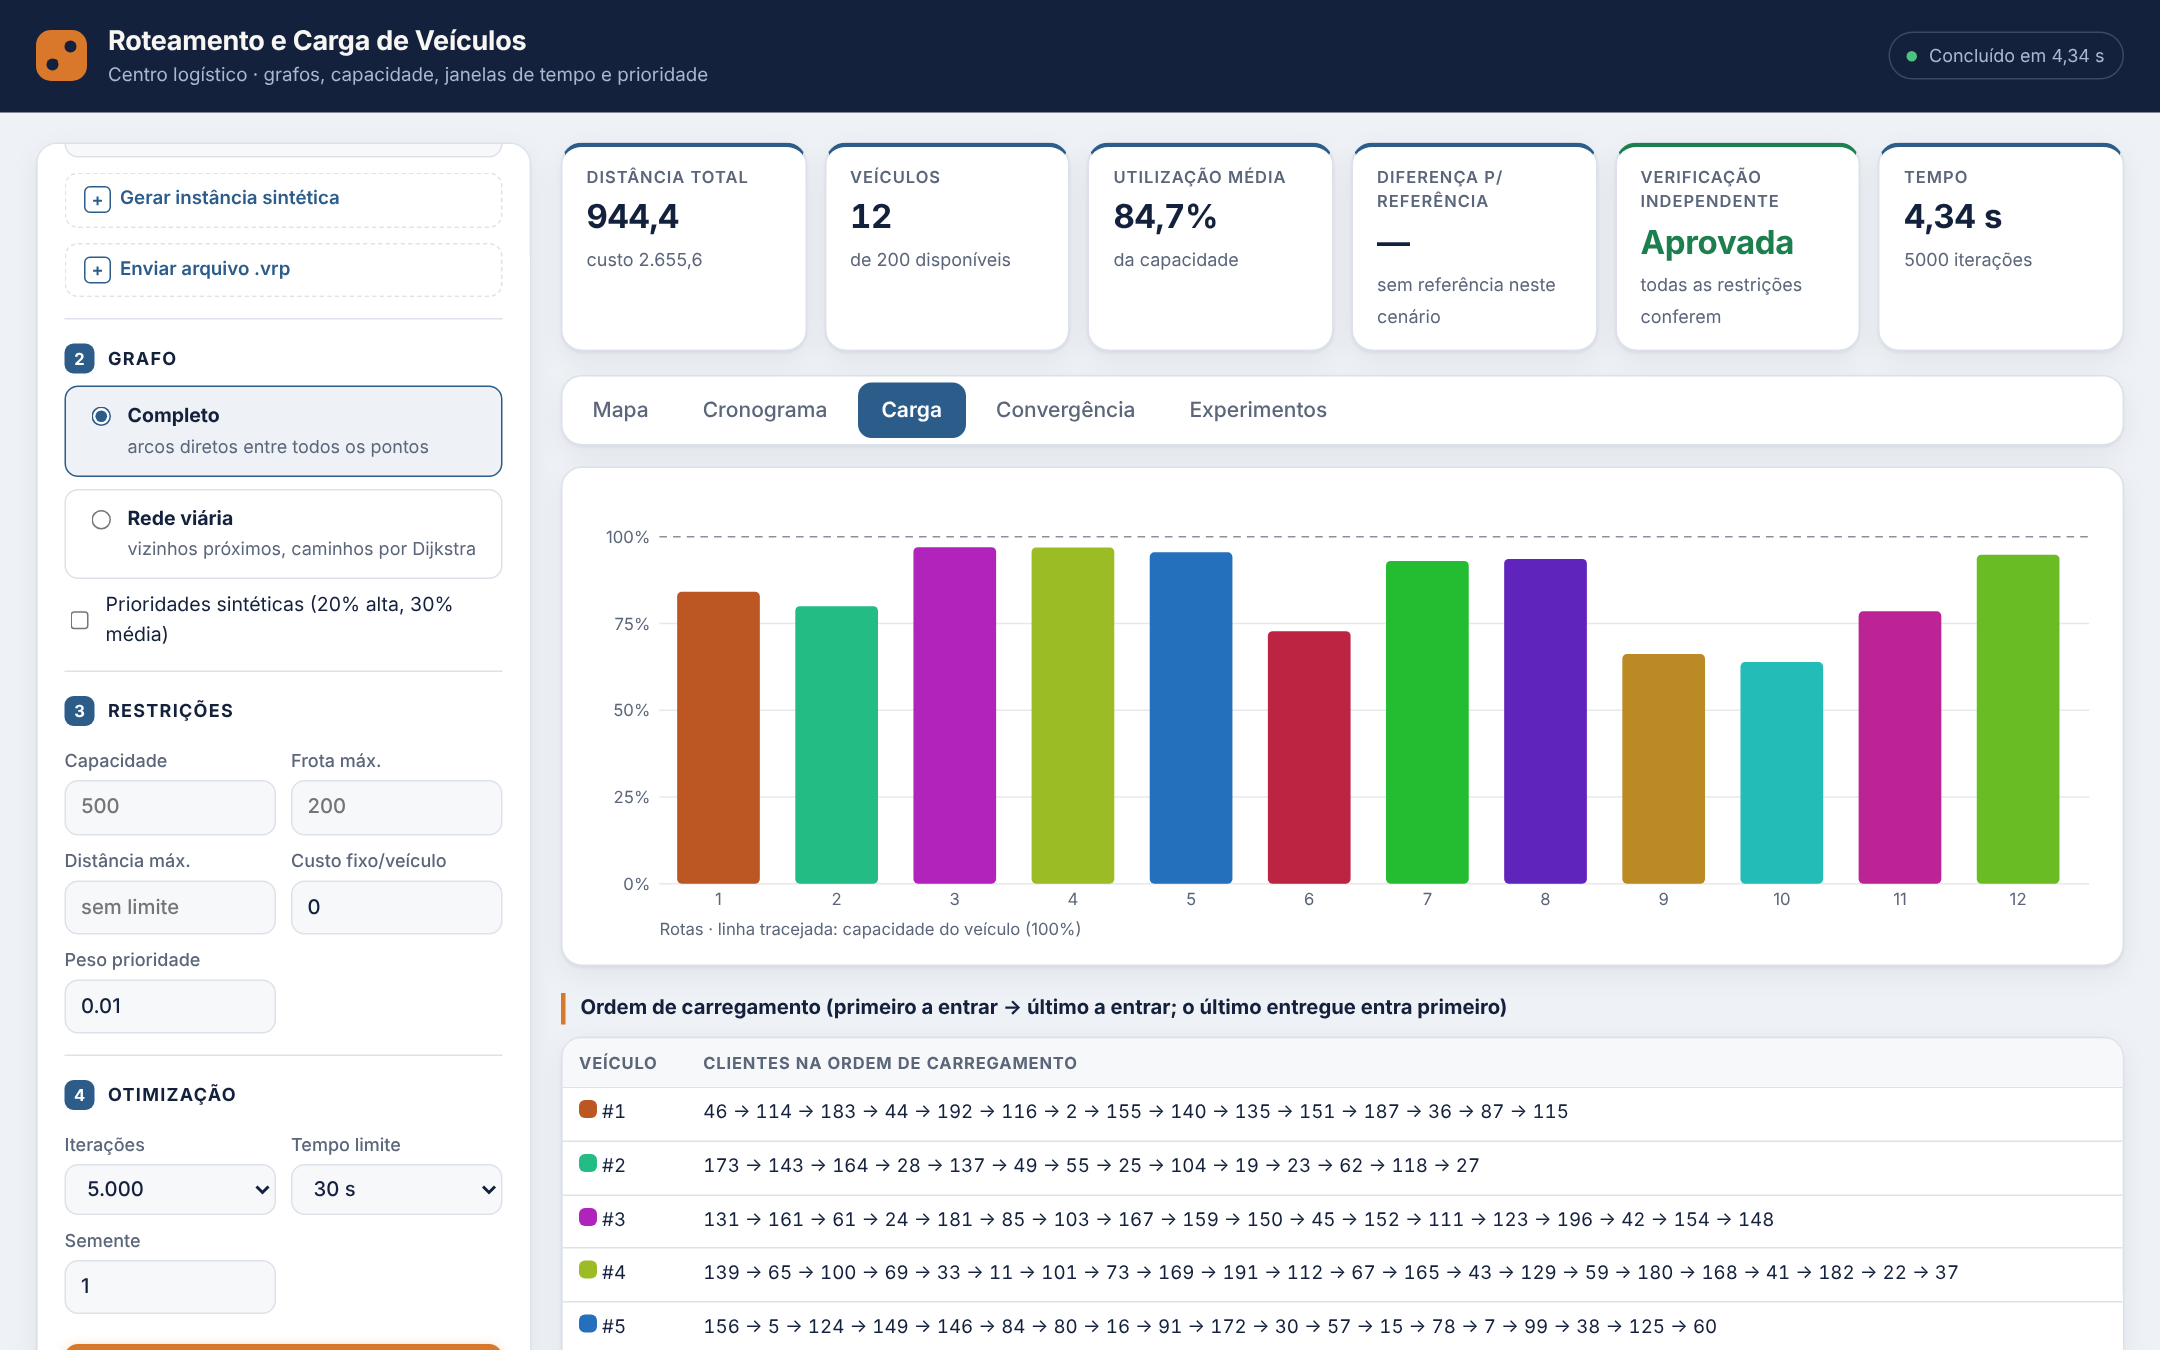
\includegraphics[width=\linewidth]{figuras/tela_carga.png}\end{minipage}
\begin{minipage}{0.325\linewidth}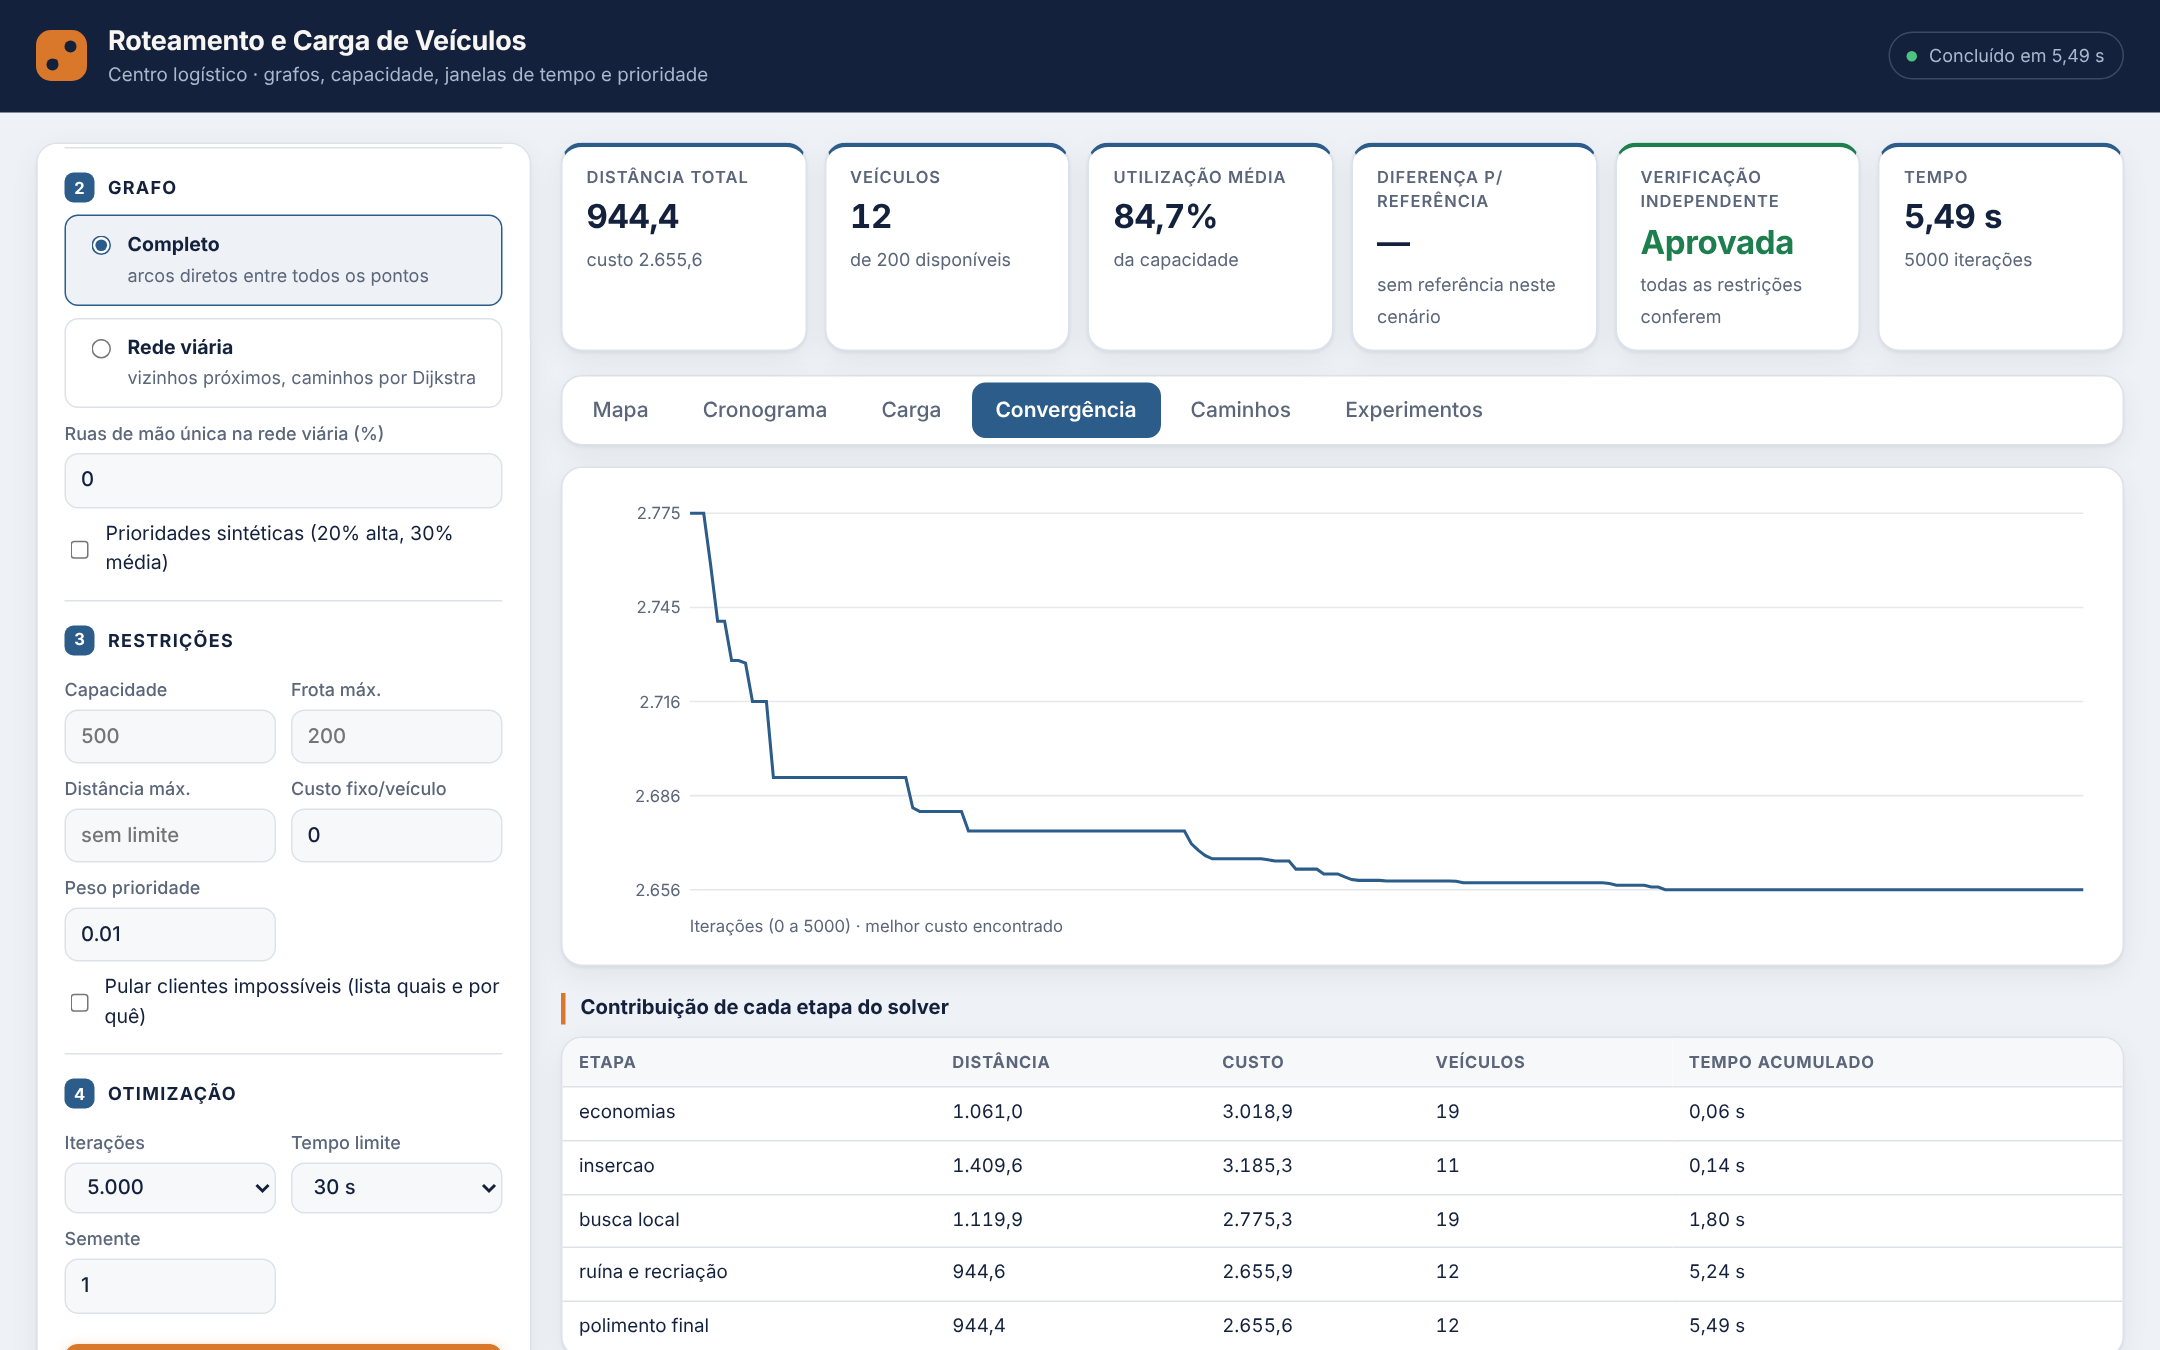
\includegraphics[width=\linewidth]{figuras/tela_convergencia.png}\end{minipage}
\begin{minipage}{0.325\linewidth}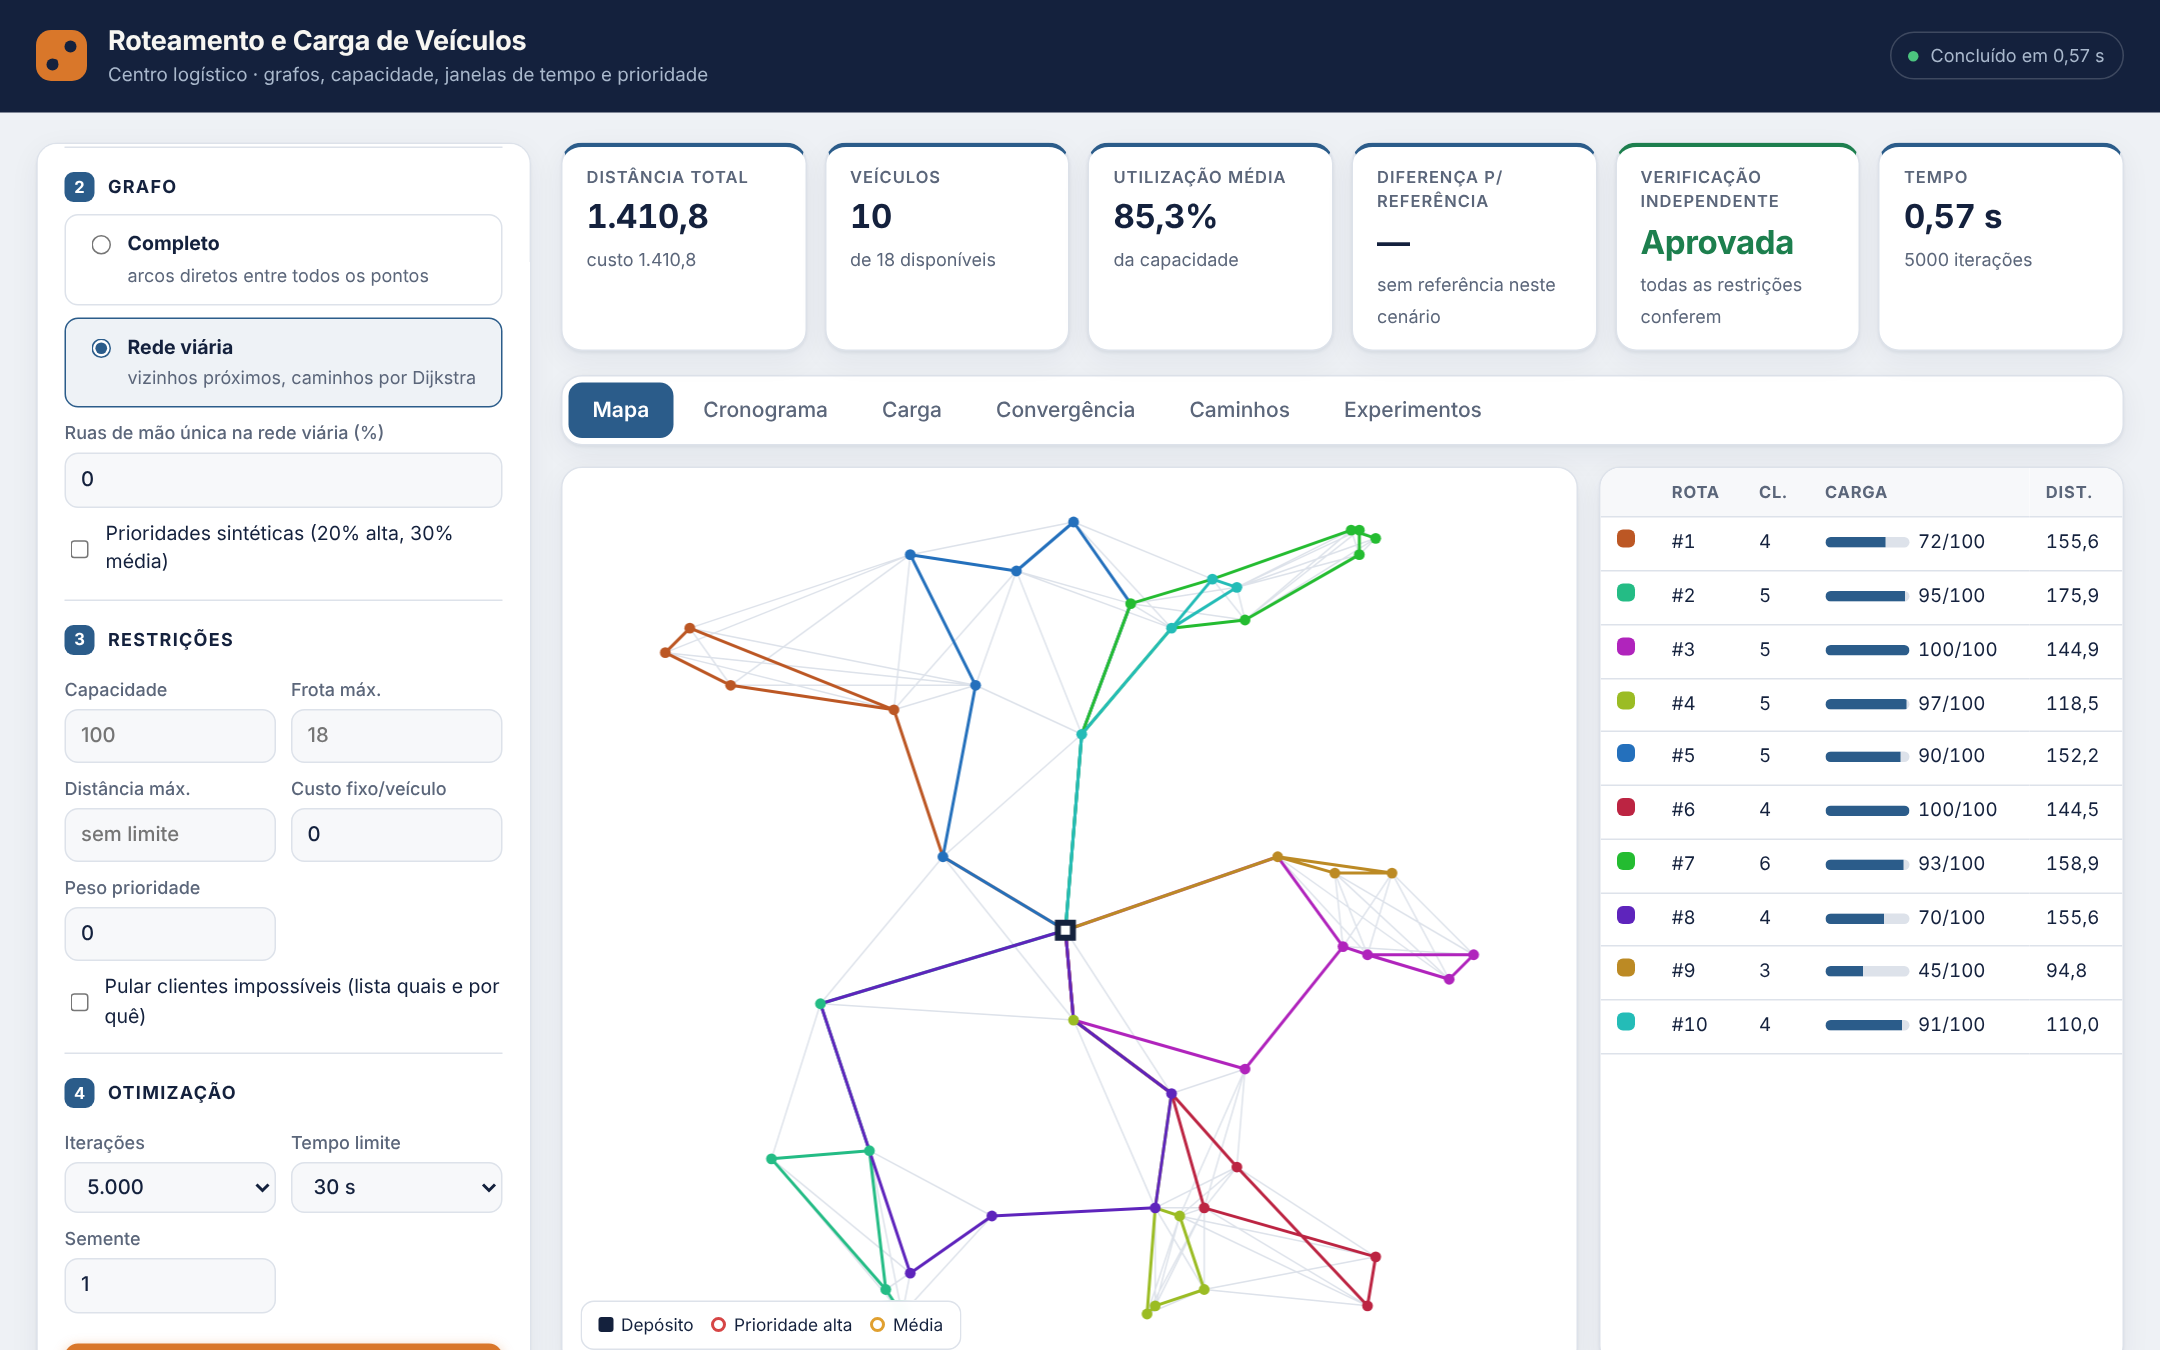
\includegraphics[width=\linewidth]{figuras/tela_viario.png}\end{minipage}
\caption{Da esquerda para a direita: carga e ordem de carregamento, convergência do custo por etapa e uma instância sintética no modo rede viária, com os trajetos físicos.}
\label{fig:telas2}
\end{figure}

\section{Validação}

A confiança no resultado vem de camadas independentes:
\begin{enumerate}
  \item \textbf{Estruturas e algoritmos de grafos.} Dijkstra é comparado com Floyd-Warshall em 60 grafos aleatórios, com pesos iguais, arestas de peso zero e vértices inalcançáveis; Kruskal, com a enumeração de todas as árvores geradoras em grafos pequenos; a alcançabilidade e as componentes, em grafos desconexos e com mão única.
  \item \textbf{Avaliação de rotas.} A inserção em tempo constante é comparada com o recálculo completo da rota em centenas de casos, com e sem prioridade e distância máxima.
  \item \textbf{BKS como referência externa.} O verificador reproduz o custo exato das 65 melhores soluções conhecidas e as aprova, o que valida leitura, arredondamento, grafo e regras de viabilidade.
  \item \textbf{Solver exato.} O próprio solver exato é conferido por enumeração completa de partições. Depois, a heurística é comparada com ele em \exN{} instâncias de 8 clientes.
  \item \textbf{Casos de falha.} Arquivo ausente ou inválido, capacidade menor que a demanda, rede desconexa, cliente impossível, frota insuficiente, requisições malformadas e tentativa de acessar arquivos fora da pasta de dados.
  \item \textbf{Reprodutibilidade.} A mesma semente e as mesmas iterações geram a mesma solução.
\end{enumerate}
O verificador detecta cliente repetido ou faltando, capacidade, janela, distância, frota e custo informado errado, cada um com teste próprio. Os testes automatizados cobrem estes itens e rodam com \texttt{python -m unittest}. Durante o trabalho a validação encontrou um defeito real, já corrigido e coberto por teste de regressão: o gerador sintético criava clientes impossíveis de atender no modo viário. A varredura final achou outro: marcar prioridades sintéticas sobrescrevia a prioridade que o arquivo do Kaggle já traz. Ela também mostrou que as economias, sozinhas, podem usar mais veículos que a frota (31 contra 25 em R101), o que o solver final trata.

\section{Resultados}

Os experimentos rodaram em um ambiente com 2 núcleos e Python 3.13, com 10\,000 iterações e semente 1 por instância; os tempos dependem da máquina, mas as distâncias não. Todas as soluções passaram na verificação independente. A diferença para a BKS é $(\text{distância}/\text{BKS}-1)\times100$, com $F=\lambda=0$. Cada instância é resolvida de forma independente, em processos paralelos, e os resultados são gravados em arquivos CSV, de onde as tabelas e figuras deste artigo são geradas automaticamente. Repetir o comando com a mesma semente reproduz as mesmas distâncias.

\subsection{Instâncias de Solomon}

Nas \solN{} instâncias (Tabela~\ref{tab:sol} e Figura~\ref{fig:gapsol}), a diferença média foi \solGapMedio\%, a mediana \solGapMediana\% e a máxima \solGapMax\% (\solPior). Em \solIgual{} instâncias a BKS foi igualada. Todas as \solVerificadas{} soluções foram aprovadas. O tempo médio foi de \solTempoMedio{} s por instância. O solver usou \solVeicSolver{} veículos no total contra \solVeicBks{} das BKS: a BKS considerada minimiza distância, e o solver segue o mesmo objetivo, sem priorizar a frota.

\begin{table}[!ht]
\centering
\small
\tabSolomon
\caption{Instâncias de Solomon por família. A família C é agrupada, R é aleatória e RC é mista; 1 e 2 indicam horizonte curto e longo.}
\label{tab:sol}
\end{table}

\begin{figure}[!ht]
\centering
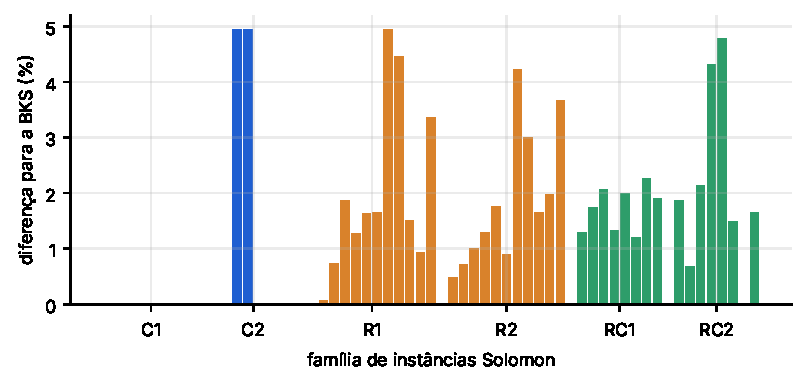
\includegraphics[width=0.75\linewidth]{figuras/fig_gap_solomon.pdf}
\caption{Diferença para a melhor solução conhecida em cada instância de Solomon.}
\label{fig:gapsol}
\end{figure}

\subsection{Instâncias do conjunto X}

Nas \xN{} instâncias sem janelas, de 101 a 303 clientes (Tabela~\ref{tab:cvrp}), a diferença média foi \xGapMedio\% e a máxima \xGapMax\%, com \xVerificadas{} soluções aprovadas. A diferença cresce com o tamanho, como se espera de uma heurística com orçamento fixo de iterações. Como nenhuma delas tem janelas de tempo, esse conjunto exercita apenas capacidade e frota, e serve de contraponto às instâncias de Solomon, em que as janelas também restringem as rotas.

\begin{table}[!ht]
\centering
\small
\tabCvrp
\caption{Instâncias CVRP-X: solver contra a BKS (distância).}
\label{tab:cvrp}
\end{table}

\subsection{Dados do Kaggle}

\textbf{Gehring-Homberger.} Rodamos a primeira instância de cada uma das seis famílias nos cinco tamanhos, 30 instâncias, todas aprovadas pelo verificador. Até 400 clientes foi usado o solver completo, com melhoria de \ghMelhoriaMin\% a \ghMelhoriaMax\% sobre a construção inicial; de 600 a 1000 clientes, a construção e a busca local, sem a ruína e recriação, com melhoria de \ghBuscaMelhoriaMin\% a \ghBuscaMelhoriaMax\% em no máximo \ghTempoMaxBusca\,s por instância. A Tabela~\ref{tab:gh} compara as instâncias de 200 clientes com as BKS do SINTEF\footnote{\url{https://www.sintef.no/projectweb/top/vrptw/200-customers/}}. Em C1 e C2 o solver iguala a BKS, com o mesmo número de veículos. Nas demais famílias ele usa mais veículos, e a comparação de distância não vale: a BKS minimiza primeiro o número de veículos e depois a distância, enquanto o nosso objetivo é a distância. Por isso, em R2 e RC2, a distância do solver é até menor que a da BKS.

\begin{table}[!ht]
\centering
\small
\tabGH
\caption{Gehring-Homberger de 200 clientes contra a BKS; ``---'' quando o número de veículos difere.}
\label{tab:gh}
\end{table}

\textbf{Entregas de e-commerce.} O arquivo não traz depósito: usamos o centroide das entregas. Latitude e longitude viram quilômetros por projeção equirretangular, a demanda é o peso do pedido, a capacidade é de 500\,kg, a velocidade é de 35\,km/h (média da coluna de velocidade), o início da janela é a hora do dia e o fim é o início mais a duração informada. A prioridade 1 é tratada como alta, 2 como média e 3 ou 4 como baixa, uma suposição nossa, pois o arquivo não define o sentido da escala. Com $\lambda=0$ o solver só minimiza distância; com $\lambda>0$ ele antecipa as entregas prioritárias. A Tabela~\ref{tab:ent} mostra o atraso médio, em minutos, entre a abertura da janela e o início do atendimento. Com $\lambda=0{,}01$ e 200 entregas, o atraso das de prioridade alta cai de \entAltaBase{} para \entAltaPrio{} minutos, com \entDistPct\% a mais de distância; com 500 entregas, de \entAltaBaseQ{} para \entAltaPrioQ{} minutos, com \entDistPctQ\% a mais. Na rede viária, 200 entregas custam \entViarioPct\% mais distância que no grafo completo. As 1000 entregas foram atendidas com \entMil{} veículos pela construção e busca local, em \entMilTempo\,s. Todas as \entVerificadas{} soluções passaram no verificador.

\begin{table}[!ht]
\centering
\footnotesize
\resizebox{\linewidth}{!}{\tabEntregas}
\caption{Entregas do Kaggle (grafo completo): efeito do peso $\lambda$ da prioridade.}
\label{tab:ent}
\end{table}

\subsection{Contribuição de cada componente}

A Tabela~\ref{tab:abl} mostra a diferença após cada etapa. A melhor construção inicial fica de \ablConstrMin\% a \ablConstrMax\% acima da BKS; a busca local leva essa diferença para \ablLocalMin\% a \ablLocalMax\%, e a ruína e recriação, para \ablFinalMin\% a \ablFinalMax\%. Em todas as instâncias da tabela, \ablNuncaPiorou. Nas instâncias de Solomon C101 e C201 a inserção sequencial já iguala a BKS, e nas demais a ruína e recriação dá a maior parte do ganho.

\begin{table}[!ht]
\centering
\small
\tabAblacao
\caption{Diferença para a BKS (\%) após cada etapa do solver.}
\label{tab:abl}
\end{table}

\subsection{Escalabilidade}

A Tabela~\ref{tab:esc} e a Figura~\ref{fig:esc} medem o tempo em instâncias sintéticas de 25 a 400 clientes. O grafo completo tem $O(n^2)$ arcos e a rede viária só $O(n)$ (\viarioArcosViario{} contra \viarioArcosCompleto{} arcos com 80 clientes). Os expoentes ajustados aos tempos medidos foram \expCompleto{} para construir o grafo completo, \expViario{} para a rede viária com Dijkstra, \expConstr{} para as construções com busca local e \expIter{} para mil iterações de ruína e recriação. A busca local é o gargalo prático e cresce mais rápido que a análise por iteração sugere, porque cada passada examina todas as realocações e trocas; para milhares de clientes seria preciso limitar as vizinhanças, o que não foi feito. Na verificação independente, \escalaTodasVerificadas.

\begin{table}[!ht]
\centering
\scriptsize
\setlength{\tabcolsep}{3pt}
\tabEscala
\caption{Tempos em segundos por fase, em instâncias sintéticas.}
\label{tab:esc}
\end{table}

\begin{figure}[!ht]
\centering
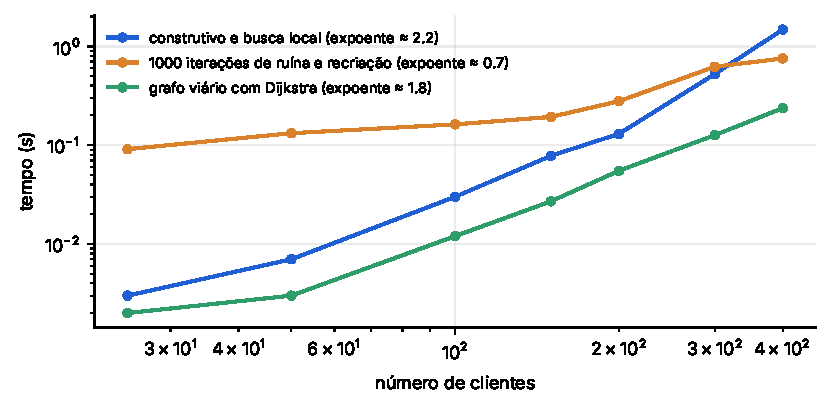
\includegraphics[width=0.75\linewidth]{figuras/fig_escala.pdf}
\caption{Tempo por fase em função do número de clientes (escala logarítmica); o expoente é o coeficiente angular ajustado.}
\label{fig:esc}
\end{figure}

\subsection{Grafo completo contra rede viária}

Em \viarioN{} instâncias sintéticas de 80 clientes, resolver na rede viária aumentou a distância total em \viarioAcrescimoMedio\% em média (de \viarioAcrescimoMin\% a \viarioAcrescimoMax\%) em relação ao grafo completo, o que é esperado, pois os caminhos têm desvio e passam por vértices intermediários. Todas as \viarioVerificadas{} soluções do modo viário foram aprovadas pelo verificador, que usa Bellman-Ford em vez de Dijkstra. A rede é gerada com os $k=5$ vizinhos mais próximos e uma árvore geradora mínima, o que garante conectividade, e cada trecho físico percorrido é desenhado no mapa.

\subsection{Efeito da prioridade}

Em \prioInstancias{} instâncias sintéticas de 60 clientes com prioridades atribuídas, variou-se $\lambda$ de 0 a \prioPesoMax{} (Tabela~\ref{tab:prio} e Figura~\ref{fig:prio}). Sem janelas de tempo, o início médio dos clientes de prioridade alta caiu de \prioSemAltaZero{} para \prioSemAltaMax{}, a soma ponderada dos inícios caiu \prioSemPondPct\% e a distância média subiu \prioSemDistPct\%. Com janelas de tempo o efeito é pequeno: o início médio da prioridade alta foi de \prioJanAltaZero{} para \prioJanAltaMax{} (a soma ponderada caiu \prioJanPondPct\% e a distância subiu \prioJanDistPct\%), porque as janelas já fixam a maior parte dos instantes de atendimento. A prioridade é, portanto, um compromisso explícito entre urgência e distância, controlado pelo usuário, e seu alcance depende da folga que as janelas deixam. Como as prioridades são sintéticas, o resultado mostra o comportamento do mecanismo e não um ganho operacional. Note que o termo penaliza todos os inícios, ponderados por 3, 2 e 1; por isso os clientes de baixa prioridade também são antecipados, em menor grau.

\begin{table}[!ht]
\centering
\small
\tabPrioridade
\caption{Efeito do peso de prioridade (médias das instâncias).}
\label{tab:prio}
\end{table}

\begin{figure}[!ht]
\centering
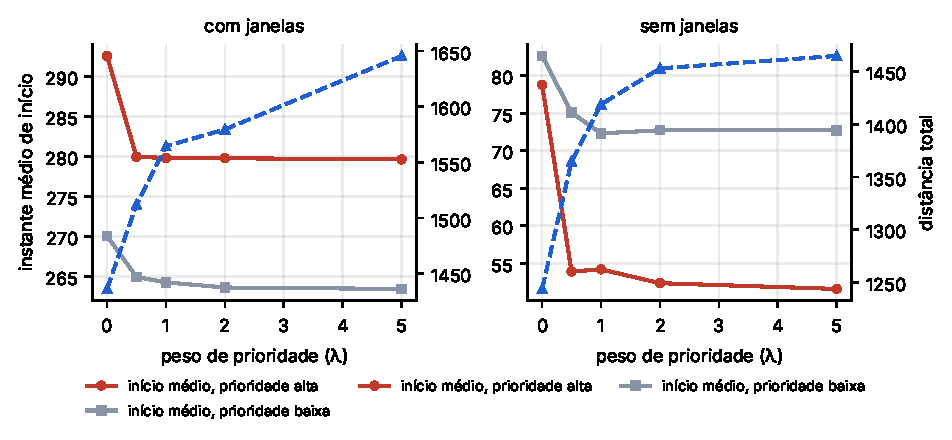
\includegraphics[width=0.8\linewidth]{figuras/fig_prioridade.pdf}
\caption{Distância e instante médio de início por prioridade, em função de $\lambda$.}
\label{fig:prio}
\end{figure}

\subsection{Heurística contra solver exato}

Em \exN{} instâncias de 8 clientes, com e sem janelas, a heurística (2\,000 iterações, uma semente) encontrou o ótimo em \exOtimas{} delas, com diferença média de \exGapMedio\% e máxima de \exGapMax\%. O solver exato levou em média \exTempoExato{} s e a heurística \exTempoHeur{} s; o tempo do exato cresce de forma fatorial com $n$ e por isso só é usado até 8 clientes. Essa concordância vale para instâncias pequenas e não garante a mesma qualidade em instâncias grandes, onde a referência são as BKS.

\section{Limitações}

\begin{itemize}
  \item A solução é heurística, sem garantia de otimalidade; a qualidade foi medida contra BKS e contra o solver exato, e este só cobre instâncias de até 9 clientes.
  \item A prioridade dos benchmarks e a rede viária são sintéticas e os tempos de viagem são iguais às distâncias (velocidade unitária). No arquivo de entregas do Kaggle a prioridade é do próprio arquivo, mas o sentido da escala, o depósito e a velocidade são suposições nossas. Os resultados desses recursos mostram o mecanismo e não a operação real.
  \item Frota homogênea, depósito único, sem coleta e entrega, sem incerteza na demanda ou no tempo de viagem.
  \item A comparação com as BKS é por distância total. As BKS de Solomon e do conjunto X usam esse mesmo critério, mas as de Gehring-Homberger minimizam primeiro o número de veículos, e por isso só comparamos distância quando ele coincide. Nas instâncias de 600 a 1000 clientes só rodamos a construção inicial.
  \item Python limita a escala: instâncias de centenas de clientes rodam em segundos a poucos minutos, e milhares de clientes exigiriam vizinhanças limitadas ou outra linguagem.
  \item As medições vêm de uma única máquina e de uma semente por instância; não foram feitos testes estatísticos entre várias sementes.
  \item Em X-n129-k18 a ruína e recriação não melhorou a solução da busca local com o orçamento usado.
\end{itemize}

\section{Conclusões}

A ferramenta modela o problema como grafo dirigido, resolve instâncias com capacidade, janelas de tempo, distância máxima e prioridade, e mostra rotas, tempos e cargas em uma interface gráfica. Em instâncias de referência ficou em média \solGapMedio\% (Solomon) e \xGapMedio\% (conjunto X) acima da melhor solução conhecida, com todas as soluções aprovadas por um verificador independente. A validação em camadas mostrou-se útil: ela revelou um defeito do gerador que o uso casual não mostraria. Como trabalhos futuros, citamos vizinhanças limitadas para instâncias maiores, tempos de viagem variáveis e dados reais de uma operação.

\section{Responsabilidades dos integrantes}

Cada integrante desenvolveu sua parte em uma branch própria do repositório, e as branches foram integradas à branch principal com merge commit, o que preserva o histórico de commits de cada um. O diagrama de casos de uso e a estrutura e o estilo da interface eram, no início, de outro integrante, que deixou a disciplina durante a Etapa~3. Essas partes foram refeitas por João Gabriel, com um visual novo e o mesmo conteúdo. A Tabela~\ref{tab:resp} resume o que cada um fez.

\begin{table}[!ht]
\centering
\small
\begin{tabular}{L{2.2cm}L{9.2cm}}
\toprule
Integrante & O que fez \\
\midrule
João Gabriel & Estrutura inicial do repositório, integração das branches na principal e commits de ajuste (arquivos fora do lugar, arquivo que faltava, READMEs de cada pasta); modelo e grafo dirigido (union-find, Kruskal, alcançabilidade); leitura das bases (VRPLIB, texto de Solomon e CSV do Kaggle) e rede viária; serviço, servidor HTTP e interface web (estrutura, estilo e lógica: mapa, cronograma, carga, convergência); diagrama de casos de uso e diagramas de classes; experimentos, figuras e tabelas; documento da Etapa 1 e relatório final \\
Pedro Eduardo & Levantamento das bases de dados; diagramas de componentes e de sequência; avaliação de rotas com folgas de tempo; heurísticas construtivas; busca local com filtros $O(1)$; ruína e recriação e solver; verificador independente; solver exato; testes com os dados do Kaggle \\
Thomas Ramos & Diagrama de atividades; caminhos mínimos com Dijkstra e seus testes; linha de comando; tutorial de uso \\
\bottomrule
\end{tabular}
\caption{Divisão das responsabilidades.}
\label{tab:resp}
\end{table}

\bibliographystyle{sbc}
\bibliography{referencias}
\end{document}
